%% This file is a portion of the source for Revised Edition 1.1 of
%% Operating Systems and Middleware: Supporting Controlled
%% Interaction, Copyright 2011 by Max Hailperin.  This work is
%% licensed under the Creative Commons Attribution-ShareAlike 3.0
%% Unported License. To view a copy of this license, visit
%% http://creativecommons.org/licenses/by-sa/3.0/ or send a letter to
%% Creative Commons, 171 Second Street, Suite 300, San Francisco,
%% California, 94105, USA.
\chapter{Processes and Protection}\label{processes-chapter}

\section{Introduction}

At this point, having seen both the threads that perform computations
and the virtual memory spaces in which those computations take place,
you are finally prepared to synthesize the notion of \vocab{process}.  Processes
play a central role in the view of an operating system as experienced
by most system administrators, application programmers, and other
moderately sophisticated computer users.  In particular, the technical
concept of process comes the closest to the informal idea of a running
program.

The concept of process is not entirely standardized across different
operating systems.  Not only do some systems use a different word (such as
``task''), but also the details of the definition vary.  Nonetheless,
most mainstream systems are based on definitions that include
the following:
\begin{description}
\item[One or more threads] Because a process embodies a running
program, often the process will be closely associated with a single
thread.  However, some programs are designed to divide work among
multiple threads, even if the program is run only once.  (For example,
a web browser might use one thread to download a web page while
another thread continues to respond to the user interface.)
\item[Virtual memory accessible to those threads] The word
``accessible'' implies that some sort of protection scheme ensures
that the threads within a process access only the memory for which that
process has legitimate access rights.  As you will see, the mainstream
protection approach is for each process to have its own virtual memory
address space, shared by the threads within that process.  However, I will also present an alternative, in which
all processes share a single address space, but with varying access rights to
individual objects within that address space.  In any case, the access
rights are assigned to the process, not to the individual threads.
\item[Other access rights]A process may also hold the rights to
resources other than memory.  For example, it may have the right to
update a particular file on disk or to service requests arriving over a
particular network communication channel.  I will address these
issues in Chapters \ref{persistence-chapter} and \ref{networking-chapter}.  For now, I will sketch two
general approaches by which a process can hold access
rights.  Either the process can hold a specific \vocab{capability},
such as the capability to write a particular file, or it can hold a
general \vocab{credential}, such as the identification of the user for
whom the process is running.  In the latter case, the credential
indirectly implies access rights, by way of a separate mechanism, such
as \vocabs{access control list}.
\item[Resource allocation context] Limited resources (such as space in
memory or on disk) are generally associated with a process for two
reasons.  First, the process's termination may serve to implicitly
release some of the resources it is holding, so that they may be
reallocated.  Operating systems generally handle memory
in this way.  Second, the process may be associated with a
limited resource quota or with a billing account for resource
consumption charges.  For simplicity, I will not comment on these
issues any further.
\item[Miscellaneous context] Operating systems often associate other
aspects of a running program's state with the process.  For example,
systems such as Linux and UNIX (conforming to the POSIX standard) keep
track of each process's current working directory.  That is, when any
thread in the process accesses a file by name without
explicitly indicating the directory containing the file,
the operating system looks for the file starting from the process's
current working directory.  For historical reasons, the operating
system tracks a single current working
directory per process, rather than one per thread.  Yet this state
might have been better associated with the individual threads, as it
is hard to see why a change-directory operation in one thread should upset file
operations underway in another concurrently running thread.  Because there is no
big master narrative to these items of miscellaneous context, I won't consider
them further in this chapter.
\end{description}

From this list, you can see that many of the key aspects of processes
concern protection, and these are the aspects on which I will focus.
Before diving into a consideration of various approaches to
protection, however, I will devote Section~\ref{process-api-section}
to the basics of how the POSIX process management API can be used,
such as how a thread running in one process
creates another process and how a process exits.  This section should
serve to make the use of processes more concrete.  Studying this API
will also allow you to
understand how the shell (command interpreter)
executes user commands.

After studying the basics of POSIX process management, you will spend
the remaining sections of the chapter learning various aspects of
protection.  Keep in mind that protection is a large and diverse area;
although I will introduce several different protection mechanisms in
this chapter, I will leave many topics for later chapters.  I
postpone some protection questions specific to file
systems to Chapter~\ref{persistence-chapter}.
Also, protection is intimately related to security, which I
cover in  Chapter~\ref{security-chapter}.  In particular, my emphasis
here will be on basic mechanisms.
I will defer to  Chapter~\ref{security-chapter} all questions of how
those mechanisms are deployed to enforce chosen security policies.

I will divide this current chapter's treatment of protection among three
sections.  Section~\ref{protecting-memory-section} addresses the fundamental
question of limiting each process's access to memory.  After showing
how processors provide two distinct execution modes to serve as
the foundation for any protection system, I will present
two approaches to memory protection: one with a separate address space for each process,
and one with a single address space.  Moving beyond memory protection,
Section~\ref{access-rights-section} first presents the fundamentals of
access rights, then
examines the two approaches I mentioned for representing access rights:
capabilities and the combination of credentials with access
control lists.  The assumption throughout these two sections is
that protection operates at the granularity of processes.
Section~\ref{protection-granularities-section} examines two alternatives, of finer and coarser
granularity.  The finer-grained protection approach protects parts of
processes from each other.  The coarser-grained approach, on the other
hand, protects entire simulated machines from one another, with each
simulated machine running its own operating system.

In
Section~\ref{securityAndProtectionSection}, the chapter concludes  with an examination of some of the
security issues most directly raised by material in the earlier
sections.

\section{POSIX Process Management API}\label{process-api-section}

All operating systems provide mechanisms for creating new processes,
terminating existing processes, and performing related actions.  The
details vary from system to system.  To provide a concrete example, I
will present relevant features of the POSIX API, which is used by
Linux and UNIX, including by Mac OS~X.

In the POSIX approach, each process is identified by a
\vocab{process ID number}, which is a positive integer.  Each process (with one exception) comes into 
existence through the \vocabindex{forking}{fork} of a
\foldvocab{parent}{process}.  The exception is the first process
created when the operating system starts running.  A process forks off
a new process whenever one of the threads running in the parent
process calls the \verb|fork| procedure.  In the parent process, the
call to \verb|fork| returns the process ID number of the new child
process.  (If an error occurs, the
procedure instead returns a negative number.)  The process ID number
may be important to the parent later, if it wants to exert some
control over the child or find out when the child terminates.

Meanwhile, the child process can start running.  The child process is
in many regards a copy of the parent process.  For protection
purposes, it has the same credentials as the parent and the same
capabilities for such purposes as access to files that have been opened
for reading or writing.
In addition, the child contains a copy of the parent's address space.  That
is, it has available to it all the same executable program code as the
parent, and all of the same variables, which initially have the same
values as in the parent.  However, because the address space is copied
instead of shared, the variables will start having different values in
the two processes as soon as either performs any instructions that
store into memory.
(Special facilities do exist for sharing some memory; I am speaking
here of the normal case.)  Of course, the operating system doesn't
need to actually copy each page of the address space.  It can use
\index{copy on write}copy on write (\index{COW}COW) to avoid (or at
least postpone) most of the copying.

Because the child process is nearly identical to the parent, it starts
off by performing the same action as the parent; the
\index{fork@\verb"|fork"|}\verb|fork| procedure returns to whatever
code called it.  However, application programmers generally don't want
the child to continue executing all the same steps as the parent;
there wouldn't be much point in having two processes if they behaved
identically.  Therefore, the \verb|fork| procedure gives the child
process an indication that it is the child so that it can behave
differently.  Namely, \verb|fork| returns a value of 0 in the child.
This contrasts with the return value in the parent process, which is
the child's process ID number, as mentioned earlier.

The normal programming pattern is for any {\tt fork} operation to be
immediately followed by  an \verb|if| statement that checks
the return value from \verb|fork|.  That way, the same program code can wind up
following two different courses of action, one in the parent and one
in the child, and can also handle the possibility of failure, which is
signaled by a negative return value.
The C$++$ program in Figure~\ref{forker-code} shows an example of this;
the parent and child processes are similar (both loop five times,
printing five messages at one-second intervals), but they are
different enough to print different messages, as shown in the sample
output in Figure~\ref{forker-output}.  Keep in mind that this output
is only one possibility; not only can the ID number be different, but the
interleaving of output from the parent and child can also vary from
run to run.
\begin{figure}
\begin{verbatim}
#include <unistd.h>
#include <stdio.h>
#include <iostream>
using namespace std;

int main(){
  int loopCount = 5; // each process will get its own loopCount
  cout << "I am still only one process." << endl;
  pid_t returnedValue = fork();
  if(returnedValue < 0){
    // still only one process
    perror("error forking"); // report the error
    return -1;
  } else if (returnedValue == 0){
    // this must be the child process
    while(loopCount > 0){
      cout << "I am the child process." << endl;
      loopCount--; // decrement child's counter only
      sleep(1); // wait a second before repeating
    }
  } else {
    // this must be the parent process
    while(loopCount > 0){
      cout << "I am the parent process; my child's ID is "
           << returnedValue << "." << endl;
      loopCount--; // decrement parent's counter only
      sleep(1);
    }
  }
  return 0;
}
\end{verbatim}
\caption{This C$++$ program, {\tt forker.cpp}, demonstrates process
  creation using {\tt fork}.  The program prints eleven lines of output,
  including five each from the parent and child process after the call
  to {\tt fork}.}
\label{forker-code}
\end{figure}
\begin{figure}
\begin{verbatim}
I am still only one process.
I am the child process.
I am the parent process; my child's ID is 23307.
I am the parent process; my child's ID is 23307.
I am the child process.
I am the parent process; my child's ID is 23307.
I am the child process.
I am the parent process; my child's ID is 23307.
I am the child process.
I am the parent process; my child's ID is 23307.
I am the child process.
\end{verbatim}
\caption{This sample output from the {\tt forker} program of
  Figure~\ref{forker-code} shows just one possible sequence of
  events.}
\label{forker-output}
\end{figure}
This example program also illustrates that the
processes each get their own copy of the \verb|loopCount| variable.
Both start with the initial value, 5, which was established before the
fork.  However, when each process decrements the counter, only its own
copy is affected.    In Programming Projects \ref{refactored-processes-project} and
\ref{dissimilar-processes-project}, you can write variants of this program.

In early versions of UNIX, only one thread ever ran in each process.
As such, programs that involved concurrency needed to create multiple
processes using \verb|fork|.  In situations such as that, it would be
normal to see a program like the one in Figure~\ref{forker-code}, which includes the full code
for both parent and child.  Today, however, concurrency within a
program is normally done using a multithreaded process.  This leaves
only the other big use of \verb|fork|: creating a child process to run
an entirely different program.  In this case, the child code in the
forking program is only long enough to load in the new program and
start it running.  This happens, for example, every time you type a
program's name at a shell prompt; the shell forks off a child process
in which it runs the program.  Although the program execution is
distinct from the process forking, the two are used in combination.
Therefore, I will turn next to how a thread running in a process can
load a new program and start that program running.

The POSIX standard includes six different procedures, any one of which
can be used to load in a new program and start it running.  The six
are all variants on a theme; because they have names starting with
\verb|exec|, they are commonly called the \vocab{exec family}.  Each
member of the exec family must be given enough information to find the
new program stored in a file and to provide the program with any
arguments and environment variables it needs.  The family members
differ in exactly how the calling program provides this information.
Because the family members are so closely related, most systems define
only the \index{execve@\verb"|execve"|}\verb|execve| procedure in the kernel
of the operating system itself; the others are library procedures
written in terms of \verb|execve|.

Because \index{execl@\verb"|execl"|}\verb|execl| is one of the
simpler members of the family, I will use it for an example.  The
program in Figure~\ref{execer-code} prints out a line identifying
itself, including its own process ID number, which it gets using the 
\index{getpid@\verb"|getpid"|}\verb|getpid| procedure.  Then it uses
\verb|execl| to run a program, named \index{ps@\verb"|ps"|}\verb|ps|,
which prints out information about running processes.  After the call
to \verb|execl| comes a line that prints out an error message, saying
that the execution failed.  You may find it surprising that the error
message seems to be issued unconditionally, without an \verb|if|
statement testing whether an error in fact occurred.  The reason for
this surprising situation is that members of the exec family return
only if an error occurs; if all is well, the new program has started
running, replacing the old program within the process, and so there is
no possibility of returning in the old program.
\begin{figure}
\begin{verbatim}
#include <unistd.h>
#include <stdio.h>
#include <iostream>
using namespace std;

int main(){
  cout << "This is the process with ID " << getpid()
       << ", before the exec." << endl;
  execl("/bin/ps", "ps", "axl", NULL);
  perror("error execing ps");
  return -1;
}
\end{verbatim}
\caption{This C$++$ program, {\tt execer.cpp}, illustrates how the
    procedure {\tt
    execl} (a member of the exec family) can be used to change which
    program the current process is running.  The same process ID that
    this program reports as its own is later shown by the {\tt ps}
    program as being its own, because the same process starts running
    the {\tt ps} program.  Note also the unconditional error message
    after the call to {\tt execl}; only if {\tt execl} fails does the
    calling program continue to run.}
\label{execer-code}
\end{figure}

Looking in more detail at the example program's use of
\index{execl@\verb"|execl"|}\verb|execl|, you can see that it takes
several arguments that are strings, followed by the special
\verb|NULL| pointer.  The reason for the \verb|NULL| is to mark the
end of the list of strings; although this example had three strings,
other uses of \verb|execl| might have fewer or more.  The first string
specifies which file contains the program to run; here it is
\verb|/bin/ps|, that is, the \verb|ps| program in the \verb|/bin|
directory, which generally contains fundamental programs.  The
remaining strings are the so-called ``command-line arguments,'' which
are made available to the program to control its behavior.  Of these,
the first is conventionally a repeat of the command's name; here, that
is \verb|ps|.  The remaining argument, \verb|axl|, contains both the
letters \verb|ax| indicating that all processes should be listed and
the letter \verb|l| indicating that more complete information should
be listed for each process.  As you can see from the sample output in
Figure~\ref{execer-output}, the exact same process ID that is
mentioned in the initial message shows up again as the ID of the process running
the \verb|ps axl| command.  The process ID remains the same because \verb|execl| has changed
what program the process is running without changing the process
itself.
\begin{figure}
\begin{verbatim}
This is the process with ID 3849, before the exec.
  UID   PID  ...  COMMAND
.
.
. 
    0  3849  ...  ps axl
.
.
.
\end{verbatim}
\caption{This sample output from the {\tt execer} program
  in Figure~\ref{execer-code} was made narrower and shorter by omitting many of
  the columns of output produced by the {\tt ps axl} command as well
  as many of its lines or output.
  The remaining output suffices to show that the process had process ID (\texttt{PID})
  3849 before it executed {\tt ps axl}, and that the same process became the process
  running the {\tt ps axl} command.}
\label{execer-output}
\end{figure}

One inconvenience about \verb|execl| is that to use it, you need to
know the directory in which the program file is located.  For example, the
previous program will not work if \verb|ps| happens to be installed
somewhere other than \verb|/bin| on your system.  To avoid this
problem, you can use \index{execlp@\verb"|execlp"|}\verb|execlp|.
You can give this variant a filename that does not include a
directory, and it will search through a list of directories looking
for the file, just like the shell does when you type in a command.  This
can be illustrated with an example program that combines \verb|fork|
with \verb|execlp|, as shown in Figure~\ref{launcher-code}.
\begin{figure}
\begin{verbatim}
#include <unistd.h>
#include <stdio.h>

int main(){
  pid_t returnedValue = fork();
  if(returnedValue < 0){
    perror("error forking");
    return -1;
  } else if (returnedValue == 0){
    execlp("xclock", "xclock", NULL);
    perror("error execing xclock");
    return -1;
  } else {
    return 0;
  }
}
\end{verbatim}
\caption{This C program, {\tt launcher.c}, runs {\tt xclock}
  without waiting for it.  The program does so by forking off a child process and executing
  {\tt xclock} in that child process.  The result is that {\tt xclock} continues
  to run in its own window while the parent process exits, allowing the shell from
  which this program was run to prompt for another command.}
\label{launcher-code}
\end{figure}

This example program assumes you are running the X Window System,
as on most Linux or UNIX systems. It runs {\tt xclock}, a program that
displays a clock in a separate window.  If you run the \texttt{launcher} program from a
shell, you will see the clock window appear, and your shell will
prompt you for the next command to execute while the clock keeps
running.  This is different than what happens if you type {\tt xclock}
directly to the shell.  In that case, the shell waits for the {\tt
xclock} program to exit before prompting for another command.
Instead, the example program is more similar to typing \verb|xclock &|
to the shell.  The \verb|&| character tells the shell not to wait for
the program to exit; the program is said to run ``in the background.''
The way the shell does this is exactly the same as the sample program:
it forks off a child process, executes the program in the child
process, and allows the parent process to go on its way. In the shell,
the parent loops back
around to prompt for another command.

When the shell is not given the \verb|&| character, it still forks off
a child process and runs the requested command in the child process,
but now the parent does not continue to execute concurrently.  Instead
the parent waits for the child process to terminate before the parent
continues.  The same pattern of fork, execute, and wait would apply in
any case where the forking of a child process is not to enable
concurrency, but rather to provide a separate process context
in which to run another program.

In order to wait for a child process, the parent process can invoke
the
\index{waitpid@\verb"|waitpid"|}\verb|waitpid| procedure.
This procedure takes three arguments; the first is the
process ID of the child for which the parent should wait, and the other two can be zero if
all you want the parent to do is to wait for termination.   As an example of a
process that waits for each of its child processes,
Figure~\ref{microshell-code} shows a very stripped-down shell.  This
shell can be used to run the user's choice of commands, such as
\verb|date|, \verb|ls|, and \verb|ps|, as illustrated in
Figure~\ref{microshell-output}.  A real shell would allow command line
arguments, offer background execution as an option, and provide many
other features.  Nonetheless, you now understand the basics of how
a shell runs programs.  In Programming Projects \ref{shell-project-1}
and \ref{shell-project-2}, you can add some of the missing features.
\begin{figure}
\begin{verbatim}
#include <unistd.h>
#include <stdio.h>
#include <sys/wait.h>
#include <string>
#include <iostream>
using namespace std;

int main(){
  while(1){ // loop until return
    cout << "Command (one word only)> " << flush;
    string command;
    cin >> command;
    if(command == "exit"){
      return 0;
    } else {
      pid_t returnedValue = fork();
      if(returnedValue < 0){
        perror("error forking");
        return -1;
      } else if (returnedValue == 0){
        execlp(command.c_str(), command.c_str(), NULL);
        perror(command.c_str());
        return -1;
      } else {
        if(waitpid(returnedValue, 0, 0) < 0){
          perror("error waiting for child");
          return -1;
        }
      }
    }
  }
}
\end{verbatim}
\caption{This C$++$ program, {\tt microshell.cpp}, is a stripped-down
  shell that waits for each child process.}
\label{microshell-code}
\end{figure}
\begin{figure}
\begin{verbatim}
Command (one word only)> date
Thu Feb 12 09:33:26 CST 2004
Command (one word only)> ls
microshell  microshell.cpp  microshell.cpp~
Command (one word only)> ps
  PID TTY          TIME CMD
23498 pts/2    00:00:00 bash
24848 pts/2    00:00:00 microshell
24851 pts/2    00:00:00 ps
Command (one word only)> exit
\end{verbatim}
\caption{This sample interaction shows the {\tt
  date}, {\tt ls}, and {\tt ps} commands being run within the
  {\tt microshell} from Figure~\ref{microshell-code}.}
\label{microshell-output}
\end{figure}

Notice that a child process might terminate prior to the parent
process invoking \verb|waitpid|.  As such, the \verb|waitpid|
procedure may not actually need to wait, contrary to what its name
suggests.  It may be able to immediately report the child process's
termination.  Even in this case, invoking the procedure is still
commonly referred to as ``waiting for'' the child process.
Whenever a child process
terminates, if its parent is not already waiting for it, the operating
system retains information about the terminated process until the
parent waits for it.  A terminated process that has not yet been waited for is
known as a \vocab{zombie}.  Waiting for a zombie makes its process ID
number available for assignment to a new process; the memory used to
store information about the process can also be reused.  This is known
as \vocabing{reap} the zombie.  Programming
Project~\ref{shell-project-2} contains additional information about
reaping zombies.

The exec family of procedures interacts in an interesting fashion with
protection mechanisms.  When a process executes a program file, there
is ordinarily almost no impact on the process's protection context.
Any capabilities (for reading and writing files, for example) remain
intact, and the process continues to operate with the same user
identification credentials.  This means that when you run a program,
generally it is acting on your behalf, with the access rights that
correspond to your user identification.  However, there is one
important exception.  A program file can have a special \vocab{set
user ID} (\vocab{setuid}) bit set on it, in which case, a process
that executes the program acquires the credential of the file's
owner.

Because a setuid program can check which user ran it, and can check
all sorts of other data (the time of day, for example), the
setuid mechanism provides an extremely general mechanism for granting
access rights.  You can grant any subset of your rights to any other
users you choose, under any conditions that you can program, by
writing a setuid program that tests for the conditions and then
performs the controlled access.  As a mundane example, you can create a
game program that has the ability to write into a file of high scores,
no matter who is running it, even though other users are
forbidden from directly writing into the file.  A similar program you have likely
encountered is the one you use to change your password.  That program can update a
password database that you do not have permission to directly modify.  As I will discuss in
Section~\ref{securityAndProtectionSection}, the setuid mechanism's
flexibility makes it useful for enforcing security
policies; however, I will also point out in Section~\ref{securityAndProtectionSection} that the same
mechanism is the source of many security pitfalls.  (Even ordinary
program execution, with credentials left unchanged, can be a
security problem, as I will discuss.)

At this point, you have seen many of the key elements of the
process life cycle.  Perhaps the most important omission is that I
haven't shown how processes can terminate, other than by returning
from the main procedure.  A process can terminate itself by using the
\index{exit@\verb"|exit"|}\verb|exit| procedure (in Java,
\index{System.exit@\verb"|System.exit"|}\verb|System.exit|), or it can
terminate another process using the
\index{kill@\verb"|kill"|}\verb|kill| procedure (see the documentation
for details).  Rather than exploring process programming further here,
I will move on to the mechanisms that operating systems use to protect
the memory occupied by processes.  If you want to pursue application programming further, the
notes section at the end of the chapter suggests additional reading.

\section{Protecting Memory}\label{protecting-memory-section}

Memory protection is the most fundamental barrier between processes,
as well as between each process and the operating system.  If a process could
freely write into the operating system's data structures, the
operating system would be unable to enforce any other kind of
protection.  In fact, if a process could write into the memory that holds
the operating system's instructions, the process could effectively
switch to an entirely different operating system of its own choosing.
Moreover, if processes could freely write into each
other's memory, a process without the ability to write a file (for
example) could manipulate another into doing so for it.  Thus, to
understand any other kind of protection, you need to first understand
how memory is protected.

Section~\ref{dual-mode-subsection} explains the foundation of this protection, which is the
processor's ability to switch between a restricted and an unrestricted
mode of operation.  Sections \ref{multiple-address-space-subsection} and \ref{single-address-space-subsection} explain how memory
protection can be built on that foundation in either of two ways: by
giving each process its own virtual memory address space or by giving
the processes differing access rights within a single address space.

\subsection{The Foundation of Protection: Two Processor Modes}\label{dual-mode-subsection}

Whether the operating system gives each process its own address space,
or instead gives each process its own access rights to portions of a
shared address space, the operating system needs to be privileged
relative to the processes.  That is, the operating system must be able
to carry out actions, such as changing
address spaces or access rights, that the processes themselves cannot perform.  Otherwise, the processes wouldn't be
truly contained; they could get access to each other's memory the same
way the operating system does.

For this reason, every modern processor can run in two different
modes, one for the operating system and one for the application
processes.  The names of these modes vary from system to system.  The
more privileged mode is sometimes called \vocab{kernel mode},
\vocab{system mode}, or \vocab{supervisor mode}.  Of
these, \vocab{kernel mode} seems to be in most common use, so I will
use it.  The
less privileged mode is often called \vocab{user mode}.

When the processor is in kernel mode, it can execute any instructions
it encounters, including ones to change memory accessibility, ones to
directly interact with I/O devices, and ones to switch to user mode and
jump to an instruction address that is accessible in user mode.  This
last kind of instruction is used when the operating system is ready to give a
user process some time to run.

When the processor is in user mode, it will execute normal
instructions, such as add, load, or store.  However, any attempt to
perform hardware-level I/O or change memory accessibility interrupts
the process's execution and jumps to a handler in the operating
system, an occurrence known as a \vocab{trap}.  The same sort of transfer to the operating system occurs for
a page fault or any interrupt, such as a timer going off or an I/O
device requesting attention.  Additionally, the process may directly
execute an instruction to call an operating system procedure, which is
known as
a \vocab{system call}.  For example, the process could use system
calls to ask
the operating system to perform the
\verb|fork| and \verb|execve| operations that I described in Section~\ref{process-api-section}.  System calls can also request
I/O, because the process doesn't have unmediated access to the I/O
devices.  Any transfer to an operating system routine changes the
operating mode and jumps to the starting address of the routine.  Only
designated entry points may be jumped to in this way; the process
can't just jump into the middle of the operating system at an
arbitrary address.

The operating system needs to have access to its own portion of
memory, as well as the memory used by processes.  The processes,
however, must not have access to the operating system's private
memory.  Thus, switching
operating modes must also entail a change in memory protection.  How
this is done varies between architectures.

Some architectures require the operating system to use one address
space for its own access, as well as one for each process.  For
example, if a special register points at the base of the page table,
this register may need to be changed every time the operating mode
changes.  The page table for the operating system can provide access
to pages that are unavailable to any of the processes.

Many other architectures allow each page table entry to contain two
different protection settings, one for each operating mode.  For
example, a page can be marked as readable, writable, and executable
when in kernel mode, but totally inaccessible when in user mode.  In
this case, the page table need not be changed when switching operating
modes.  If the kernel uses the same page table as the user-mode
process, then the range of addresses occupied by the kernel will be
off limits to the process.  The IA-32 architecture fits this pattern.
For example, the Linux operating system on the IA-32 allows each
user-mode process to access up to 3~GB of its 4-GB address space,
while reserving 1~GB for access by the kernel only.

In this latter sort of architecture, the address space doesn't change
when switching from a user process to a simple operating system
routine and back to the same user process.  However, the operating
system may still need to switch address spaces before returning to
user mode if its scheduler decides the time has come to run a
thread belonging to a 
different user-mode process.  Whether this change of address spaces is
necessary depends on the overall system design: one address space per
process or a single shared address space.
Sections \ref{multiple-address-space-subsection} and \ref{single-address-space-subsection}
address these alternatives.

Having described the distinction between kernel mode and user mode, I
am also now in a position to explain the three ways in which threads
can be implemented using those modes.  Figure~\ref{scan-7-1} shows the
three options in schematic form; I explain them in the following
paragraphs.
\begin{figure}
\centerline{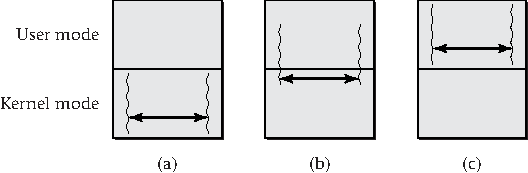
\includegraphics{hail_f0708}}
%\centerline{\def\epsfsize#1#2{0.6#1}\epsfbox{scan-7-1.eps}}
\caption{Three relationships are possible between threads, the
  scheduling and dispatching code that switches threads, and the operating modes: (a)
  the threads can be part of the kernel, along with the kernel's
  scheduler and dispatcher; (b) the threads can run mostly in user mode, but
  be scheduled and dispatched in the kernel; (c) the threads can run in
  user mode
  along with a user-level scheduler and dispatcher.}
\label{scan-7-1}
\end{figure}

As described in Chapters \ref{threads-chapter} and \ref{vm-chapter},
operating system kernels use threads for their own internal purposes,
such as zeroing out unused page frames or flushing dirty pages out to
disk. In these circumstances, the threads may execute entirely within
kernel mode; they are called \foldvocabs{kernel}{thread}.  As shown in
Figure~\ref{scan-7-1}(a), the processor can run a first kernel thread, the
kernel's scheduling and thread dispatching code, and then a second
kernel thread, all without leaving kernel mode.

An operating system kernel's scheduler may also choose to run a thread
that is part of a user-mode process.  As shown in
Figure~\ref{scan-7-1}(b), switching between user threads requires two
mode switches, even if the threads are in the same process.  First, a
switch from user mode to kernel mode is needed when moving from one
user thread to the scheduler.  Second, a switch from kernel mode back to
user mode is needed when the kernel dispatches the next user thread.
Nomenclature for these kernel-supported user threads is not
standardized; the most common term seems to be
\foldvocabs{native}{thread}, or simply \vocabs{thread} when the
context is clear.

To avoid mode-switching costs when switching threads within a process,
some middleware systems provide scheduling and dispatching mechanisms
analogous to the kernel's but residing within the user-level code,
that is, the code running in user mode.  As
shown in Figure~\ref{scan-7-1}(c), this allows the outgoing thread,
the scheduler, and the incoming thread to all execute in user mode
with no mode switch---provided the two threads are in the same
process.  These threads are commonly called
\foldvocabs{user-level}{thread}, but I prefer Microsoft's name,
\vocabs{fiber}.  This name makes clear that I am not talking about
Figure~\ref{scan-7-1}(b)'s threads, which also contain user-level code.  Moreover, the
name provides a nice
metaphor, suggesting that multiple fibers exist within one native,
kernel-supported thread.  As shown in Figure~\ref{scan-7-2}, the
kernel's scheduler divides the processor between threads, but within
each thread, there can also be a user-level scheduler switching
between fibers.
\begin{figure}
\centerline{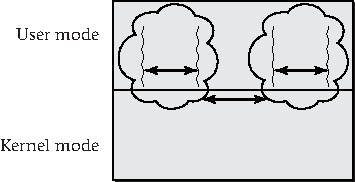
\includegraphics{hail_f0709}}
%\centerline{\def\epsfsize#1#2{0.6#1}\epsfbox{scan-7-2.eps}}
\caption{Multiple user-level threads can be enclosed in each
  kernel-supported native thread. The kernel's scheduler switches
  between the enclosing native threads.  Within each of them,
  user-level dispatching also occurs.  This creates
  what Microsoft calls fibers within the threads.}
\label{scan-7-2}
\end{figure}

Although you needed to understand the two processor modes in order to
appreciate the preceding three kinds of threads, you should keep in
mind that I introduced you to the processor modes for a different
reason.  Namely, the processor modes provide the foundation for the
protection of processes.  For example, the processor modes allow each
process to be confined within its own address space in a multiple
address space system.

\subsection{The Mainstream: Multiple Address Space Systems}\label{multiple-address-space-subsection}

Most operating systems (including Linux,
Microsoft Windows, and Mac OS~X) provide memory protection by giving each
process its own virtual memory address space.  Unless the application programmer
makes special arrangements, these address spaces are completely
disjoint.  However, the programmer can explicitly ask the operating
system to map the same file, or the same block of shared memory space,
into several processes' address spaces.

The multiple address space design is particularly appropriate on
architectures with comparatively narrow addresses.  For example, a
32-bit address can reference only a 4-GB address space.  If a 32-bit
system is going to run several processes, each of which has a couple
gigabytes of data to access, the only way to obtain enough space is by
using multiple address spaces.  This motivation for multiple address
spaces goes away (for present practical purposes) on 64-bit systems.

Regardless of address size, the multiple address space design confers
other advantages, which I mentioned in
Section~\ref{vm-intro-section}, where I provided a rationale for virtual memory.
Each process can allocate virtual addresses independently from the
others.  This means that a compiler can build addresses into a
program, even though several concurrent processes may be running the
same program; each will be able to use the pre-determined addresses
for its own copy of data.  Moreover, procedures to dynamically
allocate memory (for example, when creating objects) can work
independently in the different processes.  Even shared memory can
independently appear at the most convenient virtual address for each
process.  For example, several processes running the same program can
all consistently use one virtual address for their input channels, and
all consistently use a second virtual address for their output
channels, even if one process's output channel is another's input
channel.

However, independent address spaces can also confer disadvantages.  I
briefly mentioned one in Section~\ref{controlled-sharing-subsection}:
inconsistent virtual addresses for shared memory means pointer-based
structures can't be shared.  At the level of abstraction provided by
programming languages, objects are linked together by pointers (as
in C$++$) or references (as in Java).  At the lower level of
abstraction executed by the computer, these language constructs
generally are represented by virtual addresses; one object contains
the virtual address of another.  With separate address spaces, virtual
addresses are meaningful only within one process.  Thus, while a
shared memory region can contain a simple data structure, such as a
contiguous array of characters, it cannot contain anything complex
enough to need pointers, such as a linked list or tree.  Strictly
speaking, pointers can be used as long as they are represented other
than as virtual addresses (which most compilers won't do) or the
processes take care to map the shared memory into the same locations
(which is difficult to square with their independent allocation of
other memory).  Pointer-based data structures that span multiple
shared memory regions are even more problematic.

You can see one important variant of the pointer problem if you
recognize that memory holds code as well as data.  Instructions
sometimes include virtual addresses: either the virtual address of
another instruction to jump to or the virtual address of a data
location to load or store.  The virtual addresses included within
instructions suffer the same fate
as pointers: either they need to be kept local to one process or the
processes need to coordinate their assignments of virtual addresses.
However, if the processes need to coordinate address allocation, you have
already traded away one of the advantages of separate address spaces.
For example, consider a DLL that is mapped into several processes'
address spaces.  It would be natural if instructions within the DLL
could include the addresses of other locations within the same DLL.  However,
that is not possible unless the DLL occupies the same range of
virtual addresses within each process.

Another disadvantage to separate address spaces is that addresses
cannot be used as the ultimate system-wide name for objects. For
example, suppose two processes are communicating, and one of them
wants to suggest to the other that it map some new object into its address space.
The sending process can't specify the object in question by address (even
though it may have an address for the object), because the receiving process
doesn't yet have an address for the object.  Instead, the
communication needs to be in terms of some other, address-neutral
nomenclature, such as filenames.  Similarly, virtual addresses can't
play any role in persistent storage of objects, because their validity
is confined to a single executing process.

None of these disadvantages has been sufficiently severe as to
displace multiple address space systems from the mainstream.  However,
the disadvantages have been sufficient to cause system designers to explore the
alternative, which is for all processes to share a single address space.
Single address space systems have
even been commercially deployed---in one case with considerable success.
Therefore, I will move next to a consideration of such systems.

\subsection{An Alternative: Single Address Space
  Systems}\label{single-address-space-subsection}

There is no need to consider in detail the advantages and
disadvantages of a single address space; they are the exact opposite
of those for multiple address spaces.  Processes can share and store
addresses freely but need to coordinate on their allocation.  Instead
of rehearsing the case for and against a single address space system,
I will consider how one could still protect memory with such a system.

Beyond questions of security, memory protection is critical because
programs contain bugs.  Debugging is challenging enough even if the
result of a bug in one process always manifests itself as a symptom in
that same process.  However, without memory protection, a bug in one
process can cause a symptom in another process, because the bug
can take the form of writing into memory being used by the other
process.  This situation, in which a process's data seems to
spontaneously change as a result of a bug in an unrelated process,
is a debugging nightmare.  Thus, even in a single address
space system, processes must have varying access rights to memory.
The goal in moving to a single address space is
simply to decouple the question of accessibility from that of
addressability.  The latter concerns whether a memory location can be
named, whereas the former concerns whether the location can be read
and written.

In a multiple address space system, the processes are protected from
one another through addressability; each process will typically have
no ability to name the memory locations being used by the others.
Even when two address spaces share a particular region of memory, the
accessibility of that region is seldom modulated independently for the
individual processes.  For example, it would be rare for a
shared-memory region to be marked read-only for one process but not
another.  By contrast, the processes in a single address space system
are not separated at all by addressability; they can all name any
memory location.  Instead, the processes differ with regard to the
memory regions they have permission to read and write.

Intel's Itanium architecture contains a representative mechanism for
supporting protection in a shared address space.  Each page table
entry (in a hashed page table) contains a protection key, which is
a number.  The idea is that all pages that are to be protected
in the same way have the same key.  In particular, if a data structure
spans several pages, all the pages would have the same key.
Giving a process the right to read pages with that key would give
that process the right to read the whole structure.  A collection of at least
sixteen special registers holds protection keys possessed by the currently
executing process.  Every memory access is checked: does the process
have a key that matches the accessed page?  If not, the hardware traps
to an operating system handler, much like for a page fault.

Processes may need access to more independently protected memory
regions than the number of protection key registers.  Therefore, the
operating system will normally use those registers as only a cache of
recently accessed structures' keys, much like a TLB.  When a
protection key miss fault occurs, the operating system will not
immediately assume the access was illegal.  Instead, it will first
search a comprehensive list of the process's keys.  If the missing key
is found there, the operating system will load it into one of the key
registers and resume execution.  Only if the process truly doesn't
have the key does the operating system cope with the illegal access,
such as by terminating the process.

Each protection key register contains not only a key number, but also
a set of access control bits for read, write, and execute permissions.  Recall
that each page table entry also has access control bits.  A process
can access a page only if it has the appropriate permission in its key
register and the page table entry also allows the access.  Thus, the
page table entry can specify the maximum access for any process,
whereas the protection key registers can provide modulated access for
individual processes.  For example, a process may only be able to read
a group of pages that some other process can write.

Although single address space systems remain outside the mainstream,
at least one has proved to be commercially viable.  In the 1970s, IBM
chose the single address space design for an innovative product line, the \index{System/38}System/38,
aimed at small businesses.  In 1988,
they issued a revised version of the same basic design, the
\index{AS/400}AS/400, and in 2000 they renamed the AS/400 the
\index{iSeries}iSeries.  Whatever it may be called, the design has
proved successful; as of June 2005, IBM reports that more than 
400,000 iSeries servers are installed worldwide.

\section{Representing Access Rights}\label{access-rights-section}

In Sections \ref{capabilities-subsection} and \ref{acl-subsection}, I will present the two principle
approaches to representing access rights.  First, though, I will
use Section~\ref{access-fundamentals-subsections} to clarify the vocabulary used for discussing
protection systems.

\subsection{Fundamentals of Access Rights}\label{access-fundamentals-subsections}

A protection system controls access to \vocabs{object} by
\vocabs{subject}.  An object is whatever kind of entity needs
protection: a region of memory, a file, a service that translates
names to addresses, or anything else.  
A subject is the active entity
attempting to make use of an object; I will generally assume that it is
a process, because each thread within the process has the same access
rights.
Each kind of object has its own
repertory of \vocabs{operation} that a subject can perform on it, if
the protection system permits: for example, a memory region may have
read and write operations, whereas a naming service may have lookup,
insert, and modify operations.  Each subject is also an object,
because operations can be performed on subjects, such as the operation
of terminating a process.

Although protection mechanisms normally operate in terms of access
rights given to subjects (that is, processes within the computer), those
access rights ultimately should reflect the external authority of
human users.  To capture this notion, I will say that each subject is
acting on behalf of a \vocab{principal}. For most purposes, you can
equate the word ``principal'' with ``user.''

I use the technical word ``principal'' because occasionally the
principal will be an organization rather than an individual, and
because a server process may treat client processes as principals, for
its purposes, even though the client processes are really only
intermediaries, themselves operated by users.  The distinguishing
feature of a principal is that its rights are completely a question of
policy, not of technical mechanism.  If organizational policy directs
a web server to grant some rights to particular client web browsers
(for example, those at on-campus addresses), then it is treating those
browsers as principals.  If, on the other hand, the organizational
policy directs the web server to attempt to identify the human sitting
at the web browser and grant access rights on that basis, then the
human is the principal and the web browser is just an intermediary
subject.

As my example of a web server indicates, a subject may operate on
behalf of one principal at one time and a different principal at a
different time.  Under one scenario, the web server is operating on
behalf of on-campus browsers at some times and on behalf of off-campus
browsers at other times.  Under the other scenario, the web server is
operating on behalf of different humans at different times.  This leads
to an interesting question: what access rights should the web server have?

One common design is for the operating system's protection mechanism
to give the subject the union of all the access rights it needs for
all the principals.  The subject then has the responsibility to
enforce more specific protections.  This is standard practice with web
servers.  Consider for example a web server that is running software
that lets users read their email through web browsers.  The operating
system will typically let the mail software running on the server
access all users' stored mail all the time, regardless of who is
currently reading mail.  It is up to the server-side mail program to
make sure it only lets you read your own mail, rather than someone
else's.

In the web context, a substantial redesign would typically be
necessary if the operating system were to protect principals from each
other, rather than leaving that job to the application software, such
as the mail program.  This is because the operating system is usually
completely unaware of the principals.  Google uses the Linux operating
system on their servers, but it seems completely implausible that they
would create separate Linux user identities for each user of GMail.
Thus, there is no way that the GMail system could store your mail in a
file marked at the operating system level as owned by you and only
readable by you.

Suppose, though, we move away from the web context to a situation
where an operating system supports multiple users and runs some server
software that operates at different times on behalf of different
users.  In many organizations, file storage servers and print servers
fit this pattern.  In this context, the server software (a subject) is
again running on behalf of several users (the principals) and is
accessing files (objects) that should be constrained by
principal-specific access controls.  If the server software runs all
the time with enough access rights to be able to serve all users, then
it will need to be very carefully written and checked to make sure it
accurately enforces the desired protections.  For example, the print
server needs to be checked to make sure one user can't print another
user's files.  This wouldn't just follow as an automatic consequence
of the operating system's usual enforcement of access restrictions.

A better design would be for the operating system's protection mechanism
to allow the server to switch from one set of access rights to
another.  In this case, the subject is said to move from one
\foldvocab{protection}{domain} to another; a protection domain is
simply the set of access rights possessed by a subject.

Some subjects may also need to switch domains in order to obtain extra
access rights that would not normally be available to the principal.
I have already mentioned one form this can take.  In systems such as
Linux and UNIX, when a process executes a program that has the setuid
bit set, the process switches protection domains by taking on the
identity of the program file's owner, with all the corresponding
access rights.

At any one time, you can look at one subject (call it $S$) and
one object (call it $O$) and say that $S$ is allowed to perform
some particular set of operations on $O$.  To generalize this to the
whole system, one can picture the instantaneous state of a protection
system as an \vocab{access matrix}, with one row for each subject and
one column for each object.  The entry in row $S$ and column $O$ of
the matrix is the set of operations that $S$ can perform on $O$, as
shown in Figure~\ref{scan-7-3}.  Any
attempt by a subject to perform an operation can be checked for
legality by reference to the matrix.
\begin{figure}
\vspace{3.7em}
\[\mbox{\textbf{Subjects}}\left\{\vcenter{\vspace{-3.7em}\hbox{$\begin{array}{c||c|p{6em}|c}
\multicolumn{1}{c}{}&
\multicolumn{3}{c}{\overbrace{\hspace{10em}}^{\mbox{\textbf{Objects}}}}\\
 &\cdots&\multicolumn{1}{c|}{\mbox{\boldmath$O$}}&\cdots\\\hline\hline
 \vdots&&&\\\hline
 \lower 1.25em \hbox{\boldmath$S$}&&{\centering operations $S$\\can perform\\on
   $O$\\\vspace{-1.2em}}&\\\hline
 \vdots&&&
 \end{array}$}}\right.\]
\caption{An access matrix has one row for each subject, one column
  for each object, and entries showing which operations each subject can
  perform on each object.}
\label{scan-7-3}
\end{figure}

The access matrix in most systems is very dynamic; it gains and loses
columns and rows, and the operations listed in individual cells of the
matrix change over time.  For example, forking off a new process would
add a row and a column to the matrix, because the new process is both a
subject and an object.  If the process executes a setuid program, many
of the entries in that process's row of the matrix would change,
because the new user identity conveys different access rights to many
objects.

Some changes to the access matrix also reflect explicit protection
operations, such as making a formerly private file readable by
everyone or passing an access right held by one process to another
process.  These protection operations can themselves be regulated by
access rights listed in the access matrix, as illustrated in
Figure~\ref{access-matrix-change-permissions-figure}.
\begin{figure}
\centerline{\begin{tabular}{c||c|c|c|c}
&\boldmath$F$&\boldmath$P_1$&\boldmath$P_2$&$\cdots$\\\hline\hline
\boldmath$P_1$&change accessibility&&transfer rights&\\\hline
\boldmath$P_2$&change accessibility&&&\\\hline
$\vdots$&&&&
\end{tabular}}
\caption{An access matrix can contain rights that control changes
  to the matrix itself.  In this example, the processes $P_1$ and $P_2$
  have the right to change the accessibility of file $F$, that is, to
  change entries in $F$'s column of the access matrix.  Process $P_1$
  also has the right to transfer rights to process $P_2$, that is, to
  copy any access right from the $P_1$ row of the matrix to the
  corresponding entry in the $P_2$ row.  Notice that the representation
  of the right to transfer rights relies upon the fact that each
  subject is also an object.} 
\label{access-matrix-change-permissions-figure}
\end{figure}
Changing a
file's accessibility would be an operation on that file, contained in
some entries within that file's column of the matrix.  Normally, this
operation would not appear in every entry of the column, because only
some processes should be able to change the file's accessibility.  If
only processes $P_1$ and $P_2$ have the right to change file $F$'s
accessibility, then the corresponding change-accessibility access right
would show up in the matrix in two spots, exactly where rows $P_1$ and
$P_2$ intersect with column $F$.  Similarly, if process $P_1$ can pass
an access right along to process $P_2$, there might be an entry in row
$P_1$ and column $P_2$ conferring that transfer-rights permission.
(Recall that subjects, such as $P_2$, are also objects, and hence have
columns as well as rows.)

In order to fit common protection mechanisms into the access matrix
model, some slight contortions are necessary.  For example, many
mechanisms include access rights granted to principals (users),
independent of whether they are running any computations at the time.
Thus, it becomes necessary to add the principals themselves as subjects, in
addition to their processes.  Access rights can then go in both the
row for the principal and the rows (if any) for the processes running
on behalf of the principal.  When a principal starts running a new
process, the protection system can initialize the newly added row with
rights taken from the principal's row. Alternatively, the process can
just have rights to a special operation
on the principal object, allowing it to indirectly use the principal's
rights.
Figure~\ref{access-matrix-principal} illustrates both alternatives.
\begin{figure}
\makebox[1em]{(a)} \begin{tabular}[t]{c||c|c|c|c|c}
&\boldmath$F_1$&\boldmath$F_2$&\textit{\textbf{JDoe}}&\boldmath$P_1$&$\cdots$\\\hline\hline
\textit{\textbf{JDoe}}&read&write&&&\\\hline
\boldmath$P_1$&read&write&&&\\\hline
$\vdots$&&&&&
\end{tabular}\\[1em]
\makebox[1em]{(b)} \begin{tabular}[t]{c||c|c|c|c|c}
&\boldmath$F_1$&\boldmath$F_2$&\textit{\textbf{JDoe}}&\boldmath$P_1$&$\cdots$\\\hline\hline
\textit{\textbf{JDoe}}&read&write&&&\\\hline
\boldmath$P_1$&&&use the rights of&&\\\hline
$\vdots$&&&&&
\end{tabular}
\caption{If access rights are initially granted to a principal, such as
  \textit{JDoe}, then there are two options for how those rights can be
  conveyed to a process, such as $P_1$, operating on behalf of that
  principal.  In option (a), when the process $P_1$ is created, all of
  \textit{JDoe}'s rights are copied to $P_1$'s row of the matrix; in this
  example, the rights are to read file $F_1$ and write file $F_2$.
  In option (b), $P_1$ is given just a special right to
  indirectly use the rights of \textit{JDoe}.}
\label{access-matrix-principal}
\end{figure}

The access matrix model is very general: protections are established
by sets of operations contained in an access matrix, which include
operations to change the matrix itself.  This generality suggests that
one could construct an elegant mathematical theory of protection
systems, which would work independently from the specifics of concrete
systems.  Unfortunately, the model's generality itself
limits the results such a mathematical theory can provide.  Harrison,
Ruzzo, and Ullman showed that under very basic assumptions, the
general access matrix model can simulate a Turing machine, with the
matrix playing the role of the Turing machine's tape.  Fundamental
questions, such as whether a particular access right leaks out, turn
out to be equivalent to the halting problem and, as such, are
undecidable.  Even restricting the problems enough to render them
decidable may not make them practically solvable; for example, some
fall into the class of PSPACE-complete problems.  As explained in
the end-of-chapter notes, this classification
from computational complexity theory contains only very hard
problems for which efficient solution algorithms are unlikely to
exist.
Thus, concrete protection
systems need to be analyzed individually, rather than by reference to
general results about the access matrix model.

Access matrices can represent very different security policies,
depending on their contents.  If you focus on the operations that allow
modification of the matrix, you can distinguish two broad categories of
policies: \foldvocab{Discretionary}{Access Control} (\vocab{DAC}) and
\foldvocab{Mandatory}{Access Control} (\vocab{MAC}).

Most mainstream systems (such as Linux, Microsoft Windows, and Mac
OS~X) are usually configured to use DAC, so you are probably familiar
with that class of policies, even if you are not familiar with the name.  In a DAC
system, each object is considered to be owned by a principal; when one
of your processes creates an object (such as a file), you become its
owner.  The owner has broad rights to control the object's
accessibility.  As the owner of a file, you can choose whether to let
other users read or write the file.  In some
DAC systems, you can go even further than giving away arbitrary access rights to
your files;  you can give away transferable rights, allowing other
users to further propagate access to your files.

By contrast, an object's creator in a MAC system does not obtain
control over access rights to the object.  Instead, the access rights
are determined by an explicit security policy and can be changed only
within the parameters of that policy, often only by a designated
security officer, rather than by an ordinary user.  For example,
consider a MAC system that enforces the military policy with regard to
classified documents.  If you are using such a system and have
created a classified document, the fact that you are the creator does
not give you any special control.  You cannot choose to give access to
users who are not cleared for the document's classification level.  The only way the document
can be made readable to those users is by declassifying it, an
operation that only security officers can perform.

I will postpone further comparison between DAC and MAC systems until
Section~\ref{securityAndProtectionSection}.  Even there, I will
include only the basics, leaving more detailed treatment for
Chapter~\ref{security-chapter}.  For now, I will explain the two
techniques that are used to keep track of access rights, independent
of what sort of policy those rights are enforcing.  The first
technique is the use of capabilities, which I explain in
Section~\ref{capabilities-subsection}.  The second technique is the
use of access control lists and credentials, which I explain in Section~\ref{acl-subsection}.

\subsection{Capabilities}\label{capabilities-subsection}

A \vocab{capability} is an indirect reference to an object, much like
a pointer.  The key distinction is that a capability includes not only
the information needed to locate the object, but also a set of access
rights.  For example, two processes could possess capabilities for the
same file, but one of them might have a read-only capability to the
file, whereas the other might have a capability that permitted both
reading and writing.  A process that possesses capabilities has a
tangible representation of entries from its row of the access matrix.

Nomenclature, as always, is not standardized.  Although the word
``capability'' dates back to the mid-1960s and is popular in the
academic literature, other names are used by today's mainstream
operating systems.  Microsoft Windows refers to capabilities as
\vocabs{handle}, and POSIX systems such as Linux and UNIX refer to
them as \vocabs{descriptor}.  Continuing with the example of files, a
Windows process could have a file handle that permitted reading only,
and a Linux process could have a file descriptor that permitted
reading only.  (As you will see shortly, the handles and descriptors are
actually even more indirect than capabilities; however, for everyday
purposes, programmers can and do think about them in the same way as
capabilities.)

To further confuse matters, the designers of Linux and UNIX systems
have recently started using the word ``capability'' in a somewhat
different sense.  A capability in this new sense of the word confers
rights, but does not refer to a specific object.  For example, a
process might hold a capability that allows it to access any file, or
one that allows it to kill any process.  To distinguish the two
senses, these new object-independent capabilities are sometimes called
\foldindex{POSIX}{capability}``POSIX capabilities,'' even though the
draft standard that would have made them part of POSIX was in fact
abandoned.  I will not use the word ``capability'' in this sense.

A process can store its capabilities in either of two ways, depending
on the design of the operating system.  Most systems give each process
a special storage area just for capabilities, independent of the
normal virtual memory address space of the process.  Microsoft Windows
and the POSIX systems take this approach.  The alternative approach,
taken by \index{AS/400}\index{iSeries}the iSeries, is for a process's capabilities to be stored in normal
memory, just like any other data.

A separate storage area for capabilities is called a \vocab{C-list},
which is
short for capability list.  You will also frequently see C-lists called by system-specific
names, such as \vocab{handle tables} in Microsoft Windows
and \vocab{descriptor tables} in POSIX systems.  Systems with C-lists provide special
system calls to put entries into the C-list or otherwise operate on
it, because normal load and store operations are not applicable.
Entries in the C-list are referred to by their integer positions within
the list.  For example, an operation to read from a file takes
an integer argument, which must be the position within the C-list of a
file capability that includes the read permission.  An operation to open a
file for reading adds an entry to the C-list and returns the integer
index of that entry.

It is these integer indices into the C-list that serve as handles in
Microsoft Windows or as descriptors in POSIX.  The integers can be stored
anywhere in the process's memory; however, they do not have any
significance outside the process.  From the vantage point of 
another process, the integer would just be a useless numerical value, not
a means of accessing a capability.  This means that the integer
cannot be directly used to pass the capability through
interprocess communication or retain it in persistent storage.  In order to
pass a capability from one process to another, you need to use a
special system call.  The sending process specifies the capability to
send by its integer index, and the receiving process is notified of
its newly acquired capability as an integer index.  However, the
receiving process will in general be given a different integer than
the sending process sent, because the two processes each have their own
C-lists.  In POSIX systems, descriptors are sent using
\index{sendmsg@\verb"|sendmsg"|}\verb|sendmsg| and received using
\index{recvmsg@\verb"|recvmsg"|}\verb|recvmsg|.  For example, this
would allow a process that opened a file to pass the open file descriptor
to a second process, which could then read the file.

The capability model is incomplete as an explanation of POSIX file
descriptors.  As I will explain in Chapter~\ref{persistence-chapter},
to fully understand file descriptors, you need to consider not only
their capability-like properties, but also how the operating system
keeps track of other information associated with each open file,
especially the current position within the file for reading or
writing.  For the present chapter, however, I prefer to continue with the topic of
capabilities, explaining another option for how they can be stored.

Instead of segregating the capabilities into a C-list for each
process and forcing each process to use positions within its C-list
as surrogates for the capabilities, an operating system can give the
processes direct possession of the capabilities.  In particular, IBM
chose this approach for the \index{System/38}System/38 and carried it
forward into the \index{AS/400}AS/400 and
\index{iSeries}iSeries.  I call these nonsegregated capabilities
\foldvocabyies{addressable}{capabilit}, because they are stored within the address space.

Capabilities that are addressable values are considerably more
flexible than the C-list variety.  By storing addressable capabilities
within objects, software can use them to link several independently
protected objects together into a larger structure, just as pointers
would be used to make a more traditional structure of linked objects.
This flexibility is particularly valuable in \index{AS/400}\index{iSeries}the iSeries, because (as I
mentioned in Section~\ref{single-address-space-subsection}) it is a single address space system.

The major difficulty with addressable capabilities is how to prevent
an application program from forging them.  (Recall that in the C-list
approach, the operating system stores capabilities in memory
inaccessible to the process, so forgery is a nonissue.)  Normally the
capabilities should come from trusted system calls.  However, if the capabilities
are stored in ordinary memory locations, what is to stop a program
from writing the appropriate set of bits to look like a capability and then using that
forged capability to perform a protected operation?

Three basic approaches exist to prevent capability forgery.  The
approach used by \index{AS/400}\index{iSeries}the iSeries relies on special hardware
features.  Each memory word is supplemented by a tag bit indicating
whether the word contains part of a capability.  All normal
instructions set the bit to 0, whereas capability operations set it to
1.  Only words with their tag bits set to 1 can be used as a
capability.

An alternative approach uses cryptographic techniques to achieve a
high probability that forgeries will be detected, without needing
special hardware.  If each capability is represented by a large string
of essentially random bits, and the operating system can check whether
a given string of bits is valid, the only way to forge a capability
would be by an incredibly lucky guess.

The third approach to preventing capability forgery forces all user
programs to be processed by a trusted translator that enforces a
strong type system.  The type system prevents capability forgery the
same way as any other type error.  Interestingly,
\index{AS/400}\index{iSeries}the iSeries does put all user programs
through a trusted translator; apparently its type system is simply too
weak to function without special tagging hardware.  You will see an
example of a stronger type system providing protection in
Section~\ref{protection-within-a-process}, where I discuss the use of
the Java Virtual Machine to provide protection at a finer granularity
than operating system processes.

With \index{AS/400}\index{iSeries}the iSeries's combination of a single address space and
addressable capabilities, determining the set of all capabilities
available to a given process is not an easy job.  They are not all in
one place, unlike with a C-list.  Nor can one just scan the process's
address space looking for capabilities, because the process does not
have an individual address space.  Instead, it has access to those
portions of the shared address space that are reachable through its
capabilities.  That is, each capability the process has available leads to an object, which can in turn
contain more capabilities, leading to more objects.  Some capabilities
might lead back to already discovered objects.  Thus, to find all the
capabilities would require a general directed graph traversal
algorithm, similar to what is needed for a garbage collector.

Regardless of how easy- or hard-to-find a process's capabilities are,
one can recognize this set of capabilities as being the link to the
abstract model of protection systems, which is the access matrix.  Each
process's set of capabilities corresponds with one row of the access
matrix, because it records one subject's rights to objects.  For a
hypothetical system that provided protection purely through
capabilities, the correspondence between access matrix rows and
capability sets would be exact.  The correspondence is less direct in
real systems, which blend capability-based protection with access
control lists, a topic I consider in Section~\ref{acl-subsection}.  Because of
this hybridization of protection representations, a process's set of
capabilities holds only a portion of the contents of an access matrix
row.

In all common operating systems, capabilities can be selectively
granted but not selectively revoked.  As an example of the selective
granting of capabilities, an operating system will not allow just any
process to open up a file of private information and obtain the
corresponding capability.  (You will see in Section~\ref{acl-subsection} how the
system achieves this.)  However, once a process has the
capability---whether by successfully opening the file or by being
passed the capability by another, more privileged, process---it can
continue to operate on the file.  The file's owner cannot revoke the
capability, short of destroying the file itself.  (In POSIX systems,
the owner can't even destroy the open file, but just its contents and any
names it has.)

Several systems (such as Multics and various research systems) have
supported selective revocation, in which some capabilities to an
object can be revoked, while others remain valid.  One approach is to
keep track of the location of all copies of a capability; they can be
invalidated by overwriting them.  Another approach is to check whether
a capability is still valid each time it is used to request an
operation.  For example, if capabilities are large random strings of
bits, each object can contain a list of the valid capabilities.

Irrevocable capabilities are difficult to reconcile with system
security.  For this reason, the architects of \index{AS/400}\index{iSeries}the AS/400
made a change (relative to the original design taken from
\index{System/38}System/38) and eliminated all use of capabilities
except within the operating system itself.

The POSIX systems take a more pragmatic approach to the problem of
irrevocable capabilities.  These systems use capabilities only for
short-term storage of access rights while a process is running.  As
such, any excess access rights caused by the irrevocable capabilities
will go away when the system is rebooted, in the worst case.
Long-term storage of access rights is provided by access control
lists, which are the next topic of this chapter.

\subsection{Access Control Lists and Credentials}\label{acl-subsection}

As you have seen, a capability list collects together the access rights
held by a process.  This row-wise slice of the access matrix is
natural when considering the instantaneous rights of a process as it
executes.  However, it is much less natural when setting down (or
auditing) longer-term policy regarding access rights.  For those
purposes, most systems use a mechanism based on user credentials and
access control lists.

An \vocab{access control list} (\vocab{ACL}) is essentially a
column-wise slice of the access matrix, listing for one object what
subjects may access the object, and in what manner.  However, rather
than listing the subjects at the fine granularity of individual
processes, an ACL specifies rights for users (that is, principals) or
for named groups of users.

I can show you an example of an ACL on a Microsoft Windows system by
pulling up the Properties dialog box for a folder and selecting the Security tab on that dialog box.  The
visual form of the dialog boxes is dependent on the particular version of
Windows, but the principles apply to all modern versions.  As
shown in Figure~\ref{winacl-panel1}, this folder named
``max'' has an ACL with three
entries: two for groups of users (Administrators and SYSTEM) and one
for an individual user (myself).  In the bottom part of the dialog box, you
can see that any process running with a credential from the
Administrators group is allowed Full Control over this folder.  The
permissions (such as Full Control) listed here are actually
abbreviations for sets of permissions; to see the individual
permissions, one needs to click the Advanced button (which gives the
dialog box in Figure~\ref{winacl-panel2}) and then the View/Edit button,
producing the result shown in Figure~\ref{winacl-panel3}.  As you can
see, Full Control actually is a set of thirteen different permissions.  Some
of these permissions (those with slashes in their names) have
different interpretations when applied to folders than when applied to
files.
\begin{figure}
\centerline{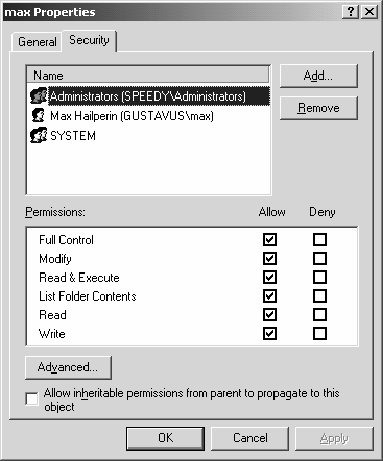
\includegraphics{hail_f0713}}
%\centerline{\def\epsfsize#1#2{0.5#1}\epsfbox{winacl-panel1.eps}}
\caption{This is the initial dialog box summarizing a Microsoft Windows
  ACL, found in the Security tab of a Properties dialog box.}
\label{winacl-panel1}
\end{figure}
\begin{figure}
\centerline{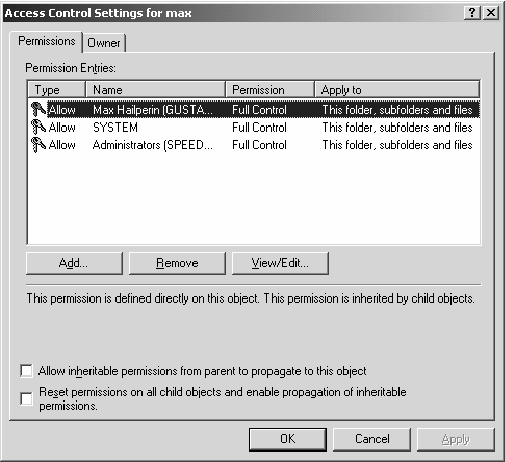
\includegraphics{hail_f0714}}
%\centerline{\def\epsfsize#1#2{0.5#1}\epsfbox{winacl-panel2.eps}}
\caption{Clicking the Advanced button on the dialog box shown in
  Figure~\ref{winacl-panel1} produces this dialog box, which in turn
  gives you the opportunity to click the View/Edit button to obtain
  the detailed view shown in Figure~\ref{winacl-panel3}.}
\label{winacl-panel2}
\end{figure}
\begin{figure}
\centerline{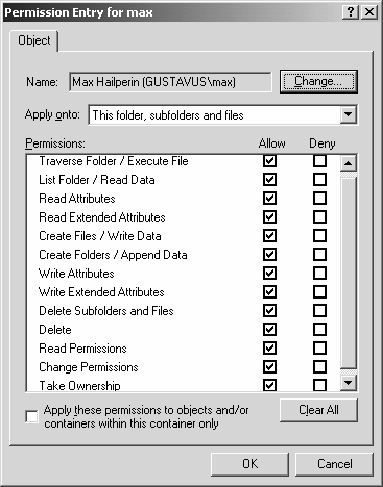
\includegraphics{hail_f0715}}
%\centerline{\def\epsfsize#1#2{0.5#1}\epsfbox{winacl-panel3.eps}}
\caption{This detailed view of a Microsoft Windows
  ACL entry allows you to see that Full Control really is a summary
  name for thirteen different permissions.}
\label{winacl-panel3}
\end{figure}

One subtlety in Figures \ref{winacl-panel1} and \ref{winacl-panel3}
concerns the presence of the Deny column of check boxes; this column is to the right of
the Allow column.  You might suspect that this is redundant, with the
Deny box checked whenever the Allow box is unchecked.  Although that
is a reasonable suspicion, it is wrong.  You can see in
Figure~\ref{winacl-panel3b} that the Users group has been neither
allowed nor denied the ability to create files in the Program Files
folder.  To understand ACLs, you need to understand the
difference between denying a permission and not allowing it.
\begin{figure}
\centerline{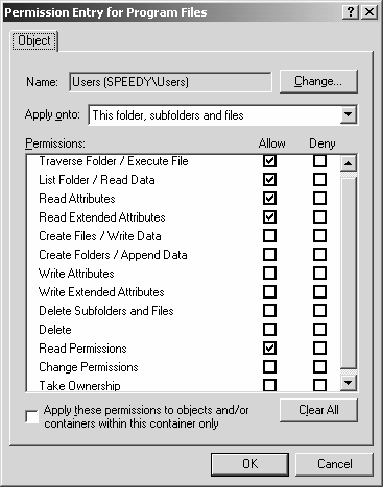
\includegraphics{hail_f0716}}
%\centerline{\def\epsfsize#1#2{0.5#1}\epsfbox{winacl-panel3b.eps}}
\caption{In the  Microsoft Windows ACL entry shown in this detailed view, some
  permissions are neither allowed nor denied.  In this circumstance,
  other ACL entries are allowed to control access.}
\label{winacl-panel3b}
\end{figure}

As you have seen, an ACL entry can allow a permission, deny it, or
neither.  (Although the graphical user interface looks as though an
entry could both allow and deny the same permission, in fact this
is not possible.  Checking one box unchecks the other.)
Keep in mind that your rights as a user derive both
from ACL entries specifically for your user identity and from other
ACL entries for groups to which you belong.  In combining together
these various ACL entries, having three options makes sense for the
same reason as in parliamentary procedure one can vote yes, no, or
abstain.  An ACL entry that abstains (neither allows nor denies a
permission) is permitting the other ACL entries to decide the
question.  In Figure~\ref{winacl-panel3b},
simply being a member of the Users group is not determinative one
way or the other with regard to creating files.  A member of the
Users group \emph{may} be able to create files in this folder,
depending on what the other ACL entries say and depending on what
other groups the user belongs to.  This is the meaning of having
neither the Allow box nor the Deny box checked.  If all applicable ACL
entries abstain, then access is denied.

What if one ACL entry that applies to a user specifies that a
permission should be allowed, while another ACL entry that also
applies to the same user specifies that the permission should be
denied?  In this case, a key difference arises between ACLs and
parliamentary procedure: the majority of the non-abstaining votes does
not win with ACLs.  Instead, a single vote to deny access will overrule
any number of votes to allow access, much like the veto power
possessed by permanent members of the United Nations Security
Council. This allows an ACL to include exceptions; for example, all
members of some group can be given access (without listing them
individually), except one specific user who is denied access.
Figure~\ref{acl-combining} summarizes the rule for combining ACL
entries.
\begin{figure}
\centerline{\begin{tabular}{l||l|l|l}
&\bf Allow&\bf Deny&\bf Neither\\\hline\hline
\bf Allow&Allow&Deny&Allow\\\hline
\bf Deny&Deny&Deny&Deny\\\hline
\bf Neither&Allow&Deny&Neither
\end{tabular}}
\caption{This table shows the rule for combining two Microsoft Windows ACL
  entries.  The same rule is used repeatedly to combine any number
  of ACL entries.  However, if the
  final result of combining all applicable entries is Neither, it is
  treated as Deny. (As the text explains, a different rule is used at
  a lower level.  This figure explains the usual interface.)}
\label{acl-combining}
\end{figure}

Within the Windows kernel, ACL entries are actually combined according to a
different rule.  If one ACL entry that applies to a user specifies that a
permission should be allowed, while another ACL entry that also
applies to the same user specifies that the permission should be
denied, the kernel obeys whichever ACL entry is listed first.
However, the API procedures that are generally used to maintain ACLs
take care that all Deny entries precede any Allow entries.  This effectively
results in the rule shown in Figure~\ref{acl-combining}, that a Deny
entry always overrides an Allow entry.  In particular, the graphical
user interface shown in the preceding figures makes use of the API
that gives precedence to Deny entries.  In
Exercise~\ref{microsoft-acl-comparison-exercise}, you can analyze the
relative merits of the two rules for combining ACL entries.

Although details vary from operating system to operating system, the
Microsoft Windows version of ACLs is typical of all systems with
full-fledged ACLs, dating back at least to Multics in the 1960s.
Rather than looking at any other examples with full ACLs, I will
consider a popular alternative, which is to use a highly restricted
form of ACL.  In particular, I will explain the file permissions
portion of the POSIX specification, implemented by Linux, Mac OS~X,
and other versions of UNIX.  (Some POSIX systems also offer the option
of full ACLs; I will focus here on the traditional, required
permission system.)

In common with Microsoft Windows, POSIX has a concept of user groups.
Each file is owned by a particular user (usually its creator) and
also has an owning group.  The ACL for any file always has exactly
three entries:
\begin{itemize}
\item
One entry specifies the permissions for the user who owns the file.
\item
The second entry specifies the permissions for all users who are members
of the owning group, except for the owning user.
\item
The third entry specifies the permissions for all other users, who are
neither the owner nor members of the owning group.
\end{itemize}
Note that unlike Windows, where several ACL entries may contribute to
a single user's permissions, only one of these three will apply to any
user.  Thus, each permission can be treated in a binary fashion
(granted or not granted), without need for the three-way distinction
of allow/deny/neither.  (Because of the way the three ACL entries are
defined, you can perform odd stunts like giving everyone but yourself
permission to access one of your files.)

Each of the three entries in a POSIX ACL can specify only three
\index{permission}permissions: read, write, and ``execute,'' which as you'll see can also
mean ``traverse directory.''  These three permissions are abbreviated
by the single letters \texttt{r}, \texttt{w}, and \texttt{x}.  A file has a total of nine
permission bits: \texttt{r}, \texttt{w}, and \texttt{x} for the owner; \texttt{r}, \texttt{w}, and \texttt{x} for the rest
of the owning group; and \texttt{r}, \texttt{w}, and \texttt{x} for everyone else. You can see
these nine bits in the output from the \verb|ls| directory listing
program, when given the \verb|-l| option (the letter \verb|l|
indicates you want a long-format listing, with lots of information).
For example, in listing my home directory, I see a line that starts with
\begin{verbatim}
drwxr-x---    4 max      mc27fac
\end{verbatim}
followed by the size, date, time, and name of the directory entry.
The letter \texttt{d} at the beginning indicates that this is an entry for a
subdirectory.  The next nine characters are the permissions; I have
full \texttt{rwx} permission, the other members of group \texttt{mc27fac} have only \texttt{r} and
\texttt{x} (but not \texttt{w}), and other users have no permissions at all.

For an ordinary file, the \texttt{rwx} permissions are relatively
self-explanatory.  However, many people are confused as to what they mean
for directories.  For a directory:
\begin{itemize}
\item
The \texttt{r} permission allows its possessor to find out what names are
listed in the directory.  This permission is neither necessary nor
sufficient to get access to one of those named files.  With only the \texttt{r}
permission on one of your directories, another user would just be able
to observe your taste in filenames.
\item
The \texttt{w} permission allows its possessor to create, delete, or rename
files in the directory.  Note, in particular, that a user who doesn't
have permission to write into one of your files may still have
permission to delete the file and create a new one with the same name.
\item
The \texttt{x} permission allows its possessor to use a filename in the
directory as part of getting access to a file, subject to that file's
own permissions.  The \texttt{x} permission allows a user to
\vocab{traverse} a directory, that is, to look up a given name in the
directory and determine what it is a name for.
Even without the \texttt{r}
permission, a user can access one of the files in
the directory if the user already knows (or can guess) its name, has the
appropriate permission to the file itself, and has the \texttt{x} permission.
\end{itemize}

As a simple rule, you should always use the \texttt{r} and \texttt{x} permissions
together on directories, unless you really know what you are doing.
Giving \texttt{x} permission without \texttt{r} can be very frustrating, because it will
break many modern programs with graphical user interfaces. These interfaces
present users with a list of files to pick from, rather than making
the user type the filename in.  The only value of \texttt{x} without \texttt{r} is for
security, but a security design that relies on other users not knowing
your obscure choices of filenames is probably not very wise.  On the
other hand, \texttt{x} without \texttt{r} is at least more useful than \texttt{r} without \texttt{x}.  You
would need to think quite creatively to find value in letting people
see your filenames but not make any use of them.  (In
Exercise~\ref{r-but-not-x-exercise}, you have the opportunity to be
that creative.)  For most normal
purposes, directory permissions should be \verb|rwx| (for yourself,
and sometimes for a group you really trust a lot), \verb|r-x| (for others you
want to use the directory), or \verb|---| (for others you want to keep
out).

As described in the preceding bulleted list, having \texttt{w} permission on a
directory is quite powerful, in that it allows you to delete and
replace an existing file within
that directory, even if you couldn't overwrite the file.  However,
this power can be kept in check.  Each directory has a bit, alongside the
nine \texttt{rwx} permission bits constituting the ACL, which can be used to limit the
power of the \texttt{w} permission.  If this so-called \vocab{sticky bit} is
set, then a file may be deleted from the directory only by the owner
of the file, the owner of the directory, or the system administrator.
The same limitation applies to renaming files.

Access control lists, of either the full variety or the simplified
owner-group-other kind, are generally used in conjunction with
capabilities.  When a POSIX process wants to read or write a file, for
example, it starts by using the \verb|open| procedure to translate the
filename into a file descriptor, which refers to a capability.

The \index{open@\verb"|open"|}\verb|open| procedure takes as arguments both the filename (a
string) and an integer encoding a set of flags.  That set of flags
contains information as to whether the process intends to read the
file, write the file, or both.  For example,
\verb|open("alpha/beta", O_RDONLY)| would attempt to obtain a read-only
capability for the file named \verb|beta| in the directory named
\verb|alpha| in the current directory.

The \verb|open| procedure uses the process's user and group
credentials to check whether the process has the necessary
permissions: \verb|x| permission on the current directory and the
subdirectory named \verb|alpha|, and \verb|r| permission on the file
named \verb|beta| within \verb|alpha|.  If the process has executed a setuid
program, these permission checks are done using the
effective user ID, adopted from the program's ownership
information.  Similarly, the permission checks take the effective
group ID from the program's owning group
if an analogous \vocab{set group ID} (\vocab{setgid})
feature is used.  Assuming the permissions are granted, the \verb|open|
procedure creates a read-only capability for the file and returns an
integer file descriptor providing access to that capability.  From
this point on, the ACLs cease to be relevant.  The \verb|x| bit could
be removed from \verb|alpha| or the \verb|r| bit from \verb|beta|, and
the open file descriptor would continue to function.  That is, an open
file descriptor is an irrevocable capability, as described in
Section~\ref{capabilities-subsection}.

\section{Alternative Granularities of Protection}\label{protection-granularities-section}

Sections \ref{protecting-memory-section} and
\ref{access-rights-section} showed how an operating system can protect
processes from unwanted interaction with one another.
Section~\ref{protection-within-a-process} considers the
possibility of providing analogous control over interaction even
within a single process, and
Section~\ref{virtual-machines-subsection} considers protecting entire
operating system environments from one another, within a single
computer.

\subsection{Protection Within a Process}
\label{protection-within-a-process}

When I described what a process is, I indicated that it is the unit
of granularity for protection provided by the operating system.  That
is, operating systems protect processes from each other, but generally
do not protect components within a process from each other.  This does
not mean that protection within a process isn't important or can't be
achieved. Instead, such protection is normally a job for middleware, rather
than for the operating system.

Consider, for example, the Java objects and threads that are used in application
servers.  Because a considerable amount of infrastructure can be safely shared
among the running instances of
web-based applications, and because instances are frequently created and later terminated,
you wouldn't want to pay the overhead cost of an
operating system process per application instance.  Instead, application servers
allow numerous instances to exist
within a single operating system process.  On the other hand, an
application server may contain applications
from many different sources.  If they were not protected from one
another, you would have the same sort of debugging and security
nightmares that you would have if processes were unprotected.

In order to protect applications from one another, even if they
coexist within a single process, the process runs the \vocab{Java
Virtual Machine} (\vocab{JVM}), which provides protection and other
basic support for Java objects and threads.  Thus, the JVM provides a good example
of how middleware can provide protection for components within a
process.

To protect Java threads, the JVM makes sure that the
Java code it is executing obeys certain restrictions.  A typical restriction is that no
method may ever read from an uninitialized local variable, that is, one
into which it has not previously written.  This prevents the method
from picking up some value left in memory by a previously executed
method, which might have been in a different application instance. 

In principle, the JVM could enforce its restrictions by carefully
monitoring each step of the Java program as it is executing.  For
example, the JVM could maintain a set of initialized local variables
as the program runs.  Any assignment to a local variable would add
it to the set.  Any use of a local variable would be preceded by a
check whether the variable is in the set.

The problem with this approach is that it would make all Java code run
like molasses in winter.  Each instruction in the program would be
preceded by hundreds of other instructions checking whether various
restrictions were satisfied.  As such, the program would be running
hundreds of times more slowly.

Therefore, real JVMs take a smarter approach.  As each class is
loaded, a JVM component called the \vocab{verifier}
mathematically proves that everywhere along all paths through the code,
no uninitialized variable is ever read.  The verifier also checks
other restrictions similarly.  Having proved that all paths are safe (in the checked
senses), the JVM can then run the code full speed ahead.

The verifier cannot check potential paths through the code one
by one, because there may be a great number of paths, or even
infinitely many.  (Consider, for example, a method with a \verb|while|
loop in the middle.  There is one path from the beginning of the
method to the end that goes around the loop zero times, one that goes
around the loop one time, and so forth.)  Therefore, the verifier constructs
its safety proofs using the same sort of dataflow analysis that
compilers have traditionally used for optimization.  This analysis
involves finding the greatest fixed-point solution of a system of
simultaneous equations.  An important general theorem regarding
dataflow analysis shows that the greatest fixed-point solution gives a
set of security guarantees that can be counted on to hold at a point,
independent of which path is taken to that point.  Therefore, the
verifier can check all paths for safety at once.  In
Exercise~\ref{jvm-verifier-exercise}, you will prove this theorem.

\subsection{Protection of Entire Simulated Machines}\label{virtual-machines-subsection}

You have seen that the JVM allows you to zoom in and create a whole collection
of protected domains within a single operating system process.
Similarly, you can zoom out and treat a whole operating system,
complete with all its processes, as just one protected domain among
many within a larger \vocab{Virtual Machine Monitor} (\vocab{VMM}).
A VMM uses the computer it runs on to simulate the execution of
several similar computers, each of which can then run its own
operating system with its own processes.

Two commercially significant VMMs are VMware's \index{ESX Server}ESX
Server and IBM's \index{z/VM}z/VM.  ESX Server uses IA-32 hardware to
simulate multiple IA-32 servers; for example, a single four-way
multiprocessor server might simulate six uniprocessor servers, each
with its own operating system, such as Microsoft Windows or Linux.
The six simulated processors take turns executing on the four real
processors, under control of the VMM.  Similarly, z/VM uses IBM's
mainframe zSeries to simulate multiple zSeries machines, each of which
could be running one of IBM's legacy mainframe operating systems or
could be running Linux.

To see how a VMM can be used, you can look at the example in
Figure~\ref{vmm-example}.
\begin{figure}
\centerline{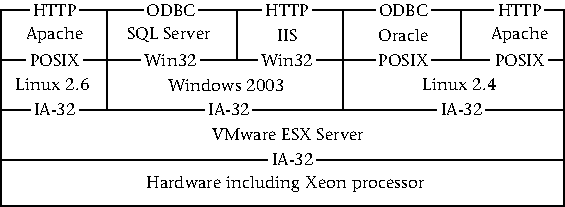
\includegraphics{hail_f0718}}
\iffalse
\centerline{\begin{graph}(350,125)
\linethickness{.02pt}
\graphnodecolour{1}
\enlargeboxes{2}
\rectnode{hardware}[350,30](175,15)
\autonodetext{hardware}{Hardware including Xeon processor}
\rectnode{VMM}[350,30](175,45)[\fillednodesfalse]
\autonodetext{VMM}{VMware ESX Server}
\rectnode{VM1}[70,30](35,75)
\autonodetext{VM1}{Linux 2.6}
\rectnode{VM2}[140,30](140,75)[\fillednodesfalse]
\autonodetext{VM2}{Windows 2003}
\rectnode{VM3}[140,30](280,75)[\fillednodesfalse]
\autonodetext{VM3}{Linux 2.4}
\rectnode{P1a}[70,30](35,105)
\autonodetext{P1a}{Apache}
\rectnode{P2a}[70,30](105,105)
\autonodetext{P2a}{SQL Server}
\rectnode{P2b}[70,30](175,105)
\autonodetext{P2b}{IIS}
\rectnode{P3a}[70,30](245,105)
\autonodetext{P3a}{Oracle}
\rectnode{P3b}[70,30](315,105)
\autonodetext{P3b}{Apache}
\textnode{hardware-VMM}(175,30){IA-32}[\graphlinecolour{1}]
\textnode{VMM-VM1}(35,60){IA-32}[\graphlinecolour{1}]
\textnode{VMM-VM2}(140,60){IA-32}[\graphlinecolour{1}]
\textnode{VMM-VM3}(280,60){IA-32}[\graphlinecolour{1}]
\textnode{VM1-P1a}(35,90){POSIX}[\graphlinecolour{1}]
\textnode{VM1-P2a}(105,90){Win32}[\graphlinecolour{1}]
\textnode{VM1-P2b}(175,90){Win32}[\graphlinecolour{1}]
\textnode{VM1-P3a}(245,90){POSIX}[\graphlinecolour{1}]
\textnode{VM1-P3b}(315,90){POSIX}[\graphlinecolour{1}]
\textnode{P1a-Net}(35,120){HTTP}[\graphlinecolour{1}]
\textnode{P2a-Net}(105,120){ODBC}[\graphlinecolour{1}]
\textnode{P2b-Net}(175,120){HTTP}[\graphlinecolour{1}]
\textnode{P3a-Net}(245,120){ODBC}[\graphlinecolour{1}]
\textnode{P3b-Net}(315,120){HTTP}[\graphlinecolour{1}]
\put(70,60){\line(0,-1){7}}
\put(210,60){\line(0,-1){7}}
\put(140,90){\line(0,-1){7}}
\put(280,90){\line(0,-1){7}}
\end{graph}}
\fi
\caption{This example shows a VMM, the VMWare ESX Server, supporting multiple operating
  systems.  The label within each box identifies a component, whereas
  the label on each horizontal dividing line identifies an interface.
  Unlike the operating systems, the VMM provides upward the same IA-32
  interface that it relies upon from below.}
\label{vmm-example}
\end{figure}
Each box indicates a hardware or software component.
At the bottom is the Xeon hardware, a member of the Pentium family,
which supplies the IA-32
interface upward to the next layer.  That next layer is a VMM
(specifically the ESX Server), which simulates three virtual machines,
each also providing the IA-32 interface.  The leftmost virtual machine
is running Linux~2.6, the middle one is running Windows~2003, and the
rightmost one is running an older version of Linux, 2.4.  The presence
of Microsoft Windows and Linux on the same hardware may have come
about through server consolidation; perhaps two different groups
within the enterprise had settled on different software environments
but now are being hosted on common hardware to reduce total cost of
ownership.  The two versions of Linux may reflect a similar story, or
may be a case where a new version is being tested while an older
version continues to be in production use.  In the particular case
shown in the figure, the Linux~2.6 virtual machine is running a single
process (the Apache web server), whereas the other two virtual
machines are running two processes apiece (in each case, a database
server and a web server).

Notice that processes can benefit from two levels of
protection, one provided by the operating system and another by the
VMM.  For example, Windows 2003 is responsible for isolating the SQL
Server process from the IIS process.  If someone finds a way to
subvert Windows's protection mechanism, this isolation may fail.
However, the processes running on the other two virtual machines will
remain isolated, so long as the ESX Server software continues to do
its job.  Consider another explanation for why two versions of
Linux are running on the same machine: one group, with a lot at stake,
might choose to run the latest version with all available security
patches, while another group, with less at stake, might choose to
stick with an older, less secure version so as to avoid the disruption
of an upgrade.  The high-stakes group need not fear consequences from
an attacker breaking into the low-stakes group's system any more than
if the two were on different hardware machines.  The VMM provides that
assurance.

The operation of a VMM is similar to that of an operating system.
Like an operating system, it uses scheduling to divide processing time
and uses page mapping to divide memory.  The key difference is that it
doesn't support any higher-level APIs, such as the file operations
found in POSIX or Win32. Instead, the VMM supports an
interface similar to a real machine's, complete with I/O devices.

Because the virtual machines use the same instruction set architecture
as the real hardware, the VMM does not need to simulate their
execution on an instruction-by-instruction basis.  Most instructions
can be directly executed by the real hardware.  The only issue is with
privileged instructions, of the kind used by operating systems for
such tasks as managing I/O hardware or changing page tables.

Recall that processors generally have two operating modes, a kernel
mode in which all instructions are legal, and a user mode, in which
dangerous instructions transfer control to a trap handler.
The trap handler is part of the software that runs in kernel mode.
I need
to explain how these two modes can be used to support three levels of
execution: the VMM, the operating system, and the application
processes.

The VMM runs in kernel mode.  When the underlying processor
executes instructions from one of the virtual machines, on the other
hand, it does so in user mode.  That way, the VMM is in complete
control and can protect the virtual machines from one another.
However, the virtual machines still need to support a simulated kernel
mode so that they can run operating systems.  Therefore, the VMM
keeps track of each virtual machine's simulated mode, that is, whether
the virtual machine is is in simulated kernel mode or simulated user
mode.

If a virtual machine executes a privileged instruction (for example,
to manage I/O hardware), a trap to the VMM occurs, as shown in
Figure~\ref{VMM-modes}.
\begin{figure}
\centerline{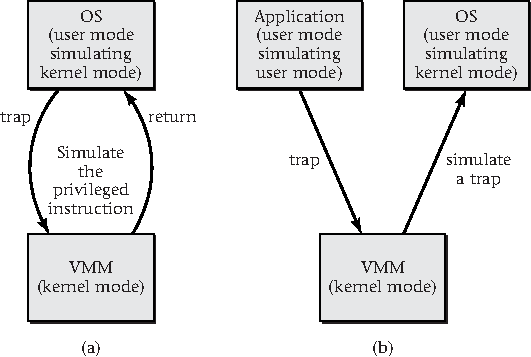
\includegraphics{hail_f0719}}
%\centerline{\def\epsfsize#1#2{0.6#1}\epsfbox{VMM-modes.eps}}
\caption{When an attempt is made to
  execute a privileged instruction within a virtual machine, a trap to the VMM occurs, whether
  the virtual machine is executing operating system code or
  application code, because the hardware is in user mode in either case.  However, the VMM
  knows whether the virtual machine is in simulated kernel mode or
  simulated user mode and responds accordingly.  In (a), the
  virtual machine is in simulated kernel mode, so the VMM simulates
  the privileged instruction and then returns from the trap. 
  In (b), the virtual machine is in simulated user mode, so the VMM
  simulates the trap that would have occurred on a real machine: it
  switches to simulated kernel mode and jumps to the operating system
  trap handler within the virtual machine.}
\label{VMM-modes}
\end{figure}
The VMM then
checks whether the virtual machine was in simulated kernel mode.  If
so, the privileged instruction was attempted by the virtual machine's
operating system, and the VMM carries out the intent of the
instruction, for example, by doing the requested I/O.  If, on the
other hand, the virtual machine was in simulated user mode, then the
VMM simulates a trap within the virtual machine by switching it to
simulated kernel mode and jumping to the trap handler within the
virtual machine's operating system.  In
Exercise~\ref{VM-trap-return-exercise}, you can consider how the trap
handler within the virtual machine's operating system can later return
control to the application program.

One particularly interesting design question is how virtual memory is
handled.  The operating system running within a virtual machine sets
up a page table mapping virtual page numbers into what it thinks of as
physical page frame numbers.  However, the VMM does another level of
mapping, translating the virtual machine's ``physical'' page frames
into the truly physical page frames of the hardware.  That way, the
VMM can allocate the hardware's memory among the virtual machines and
can do tricks like using copy on write (COW) to transparently share
memory across the virtual machines.

In order to efficiently support this double translation of addresses,
the VMM computes the functional composition of the two address
translations and provides that composition to the hardware's MMU.
That is, if the virtual machine's simulated page table would map $A$
into $B$, and the VMM wants to map $B$ into $C$, then the VMM puts a
translation directly from $A$ to $C$ into the real page table used by
the hardware MMU.

\section{Security and Protection}
\label{securityAndProtectionSection}
Protection plays an essential role in security.  If I were to take
the title of this section literally, it could be a very long section.
Instead, I will simply highlight a few key security issues directly
raised by the material in this chapter.

Perhaps the most important take-home message is that although
protection is essential to security, it is not the same as security.
The two are easily confused.  For example, security includes
maintaining confidentiality, and protection includes the use of access
control lists to limit read access permissions.  Surely these are the
same, right?  Wrong.  If the data in question is
on a disk drive that is in an unlocked room, then all the access
control lists in the world won't keep it confidential.  An adversary
simply needs to steal the drive and read it on his own machine, which
is programmed to ignore ACLs.  In Chapter~\ref{security-chapter}, I
will address some of the broader security picture.

Many nasty security pitfalls arise from the distinction between a
principal and a subject, or in simplified terms, between a
user and a process.  A process that is operating with the credentials
of a user may carry out actions that the user would not approve of.
One way this could happen is if the user authentication system is weak
enough for someone else to log in as you.  I will not consider that
topic further here, instead concentrating on the problems that remain
even if the system knows which human is behind each keyboard.

In discussing POSIX processes, I mentioned that user credentials are
retained when a process forks and also when it executes a program.
Thus, any program you run will be acting with your credentials.  (The
same is true in other systems, such as Microsoft Windows.)  This
immediately raises the possibility of a \vocab{Trojan horse}, a
program that has some apparent benign purpose but that also has a hidden nefarious intent.  Suppose
someone gives you a program and tells you it shows a really funny
animation of Bart Simpson impersonating Bill Gates.  You run it, enjoy
the animation, and chuckle merrily.  Unfortunately, you aren't the
only one laughing; so is the programmer who knows what else the program
does other than showing the animation.  Remember: whatever the program
does, ``you'' are doing, because the process is acting with your user
credentials.  If you have the ability to send all your private
data over the network (which you probably do), then so does the Trojan
horse.

One variant of the general \index{Trojan horse}Trojan horse theme is
the \foldvocab{email}{worm}.  Suppose you receive an email with an
attached program.  When you run the program, it can do anything it
wants with your credentials.  Suppose what it does is send new email
to everyone in your address book, with the same attachment. (After
all, the protection system thinks you have every right to read your
address book and to send email with your return address.)  In this
way, the same malicious program can be spread to many computers all
over the world.  Of course, the worm can perform other actions as
well.

Suppose you never knowingly run gift programs.  Does that make you
safe from \index{Trojan horse}Trojan horses?  Not necessarily; there
are a variety of ways you might unknowingly run a program.  What follows
is one example.
  Recall
my discussion of
\verb|execlp|.  I mentioned that it looks through a sequence of
directories until it finds the program file, just as the shell does.
This search means that even when you type in as simple a command as
\verb|ps| (to list your processes), you don't necessarily know what
program is being run; it might not be \verb|/bin/ps|, if some other
program named \verb|ps| is in one of the other directories that comes
before \verb|/bin| in the search path.  In particular, it was once
common for UNIX users to have search paths that started with the
current directory (named \verb|.|), before any system-wide
directories.  That has ceased to be popular, because it is an open
invitation to Trojan horses planted by adversaries who don't have
write access to any of the system-wide directories.  Even putting the
current directory last in the search path (as many users still do) is
not completely safe; a clever adversary could plant a Trojan horse
named with a common misspelling or with a program name that is
installed on some systems, but not the one under attack.  The only
really safe alternative is to leave the current directory out of your
search path.  When you want to run a program in your current
directory, you will need to specify an explicit pathname.  For
example, to run the \texttt{microshell} program from
Figure~\ref{microshell-code}, you might compile it in your current
directory and then run \verb|./microshell|.

An attacker who wants to plant a Trojan horse for you to run may not
even need to take advantage of search paths, if one of the programs
you run has file access permissions set so that other people can
overwrite the file with a modified version.  Similarly, if the
directory containing the program is writable, the program
can be deleted and replaced.  Setting programs (or the containing
directories) to be writable seems like such an obvious invitation for Trojan horses
that you might find it difficult to imagine such situations arise.
Yet I have repeatedly encountered installer
programs for commercial application software that set the installed
programs or directories to be writable by all users of the system.  In
the face of such installers, a system administrator needs to be
vigilant and manually change the permissions.  

The \index{Trojan horse}Trojan horse problem is far more dangerous in
a system with \index{Discretionary Access Control}\index{Access
Control, Discretionary}\index{DAC}Discretionary Access Control (DAC)
than one with \index{Mandatory Access Control}\index{Access Control,
Mandatory}\index{MAC}Mandatory Access Control (MAC), because there is
far more that ``you'' (actually, the Trojan horse) can do in a DAC
system.  For example, in a MAC system that enforces military
classification levels, no Trojan horse can possibly read from a
top secret file and then write a copy into an unclassified file; the
operating system forbids any process from reading and writing
in this way.  Notice that using MAC rather than DAC is only partially
intended to guard against computer users making unwise decisions.  Far
more, MAC is guarding against the organization needing to trust all
programs' authors.  (Trust in the people running the programs can come
from nontechnical sources, like keeping an eye out for employees who
seem to have too much money.  For external program authors, this would
be more difficult.)

Another security pitfall comes from the ability of a \index{set user ID}\index{setuid}setuid program to
propagate its owner's credentials.  Suppose that an adversary briefly
has the ability to act with your credentials, using some means other
than setuid.  (This could be through a Trojan horse, but alternatively
the adversary might simply use your keyboard while you are getting
coffee.)  You cannot assume that the adversary's ability to do damage
is over when the initial access method is removed (when you
return from getting coffee).  A smart adversary will use the brief
access to create a setuid shell, owned by you and executable by the adversary.
Then, at any convenient later time, the adversary can run any programs
whatsoever with your credentials.  A real-world analogy would be if
leaving your door unlocked made it easy for a burglar to retrofit a
secret entrance into your house.

System administrators fight back against unwanted \index{set user ID}\index{setuid}setuid programs with
measures such as turning the setuid feature off for file systems that
normal users can write into, as well as regularly scanning the file systems
looking for setuid files.  These measures are valuable but are
treating a symptom of a bigger problem.  The setuid mechanism, in its
elegant generality, is a fundamental mismatch for most organizational
security policies.  In most organizations, authorization can flow only
from the top down; low-level employees are not empowered to pass their
authority on to someone else.

Setuid\index{set user ID}\index{setuid} programs raise an additional
set of issues, which are in a sense the opposite of the Trojan horse
problem.  Security problems arise whenever the person providing
authority is different from the person deciding how that authority
will be used.  A Trojan horse tricks the user running the program into
providing credentials for actions specified by the program's author.
Conversely, a setuid program provides the author's credentials, but
might unintentionally allow the user running it to control what
actions it carries out.  Either way, there is a mismatch between the
source of authority and the source of control.

Programming oversights explain most cases where a \index{set user ID}\index{setuid}setuid program cedes
control to the user running it.  For example, suppose the designer of a setuid program
wants it to print out a file and wants the user running the program to
specify the name of the printer (but not of the file).
The program might execute a shell command like
\verb|lpr -P|\emph{printername}~\emph{filename}, where the
\emph{printername} comes from the user's input and the \emph{filename}
is controlled by the setuid program itself.  This seemingly innocent
command could be compromised in several ways, such as the following:
\begin{itemize}
\item
If the adversary can control the directory search path, the \verb|lpr|
command might be executing a program of the adversary's choice, rather
than the normal printing command.
\item
If the adversary can input a printer name that contains a space, the
print command might gain an extra argument, which would be taken as
another filename to print, this one specified by the adversary.
\item
If the adversary can input a printer name that contains a semicolon,
the print command might turn into two separate commands, one to run
\verb|lpr| and one to run some totally different program of the
adversary's choice.
\end{itemize}

UNIX system programmers have developed a whole body of lore on how to
write \index{set user ID}\index{setuid}setuid (or setgid) programs without falling into traps such as
the preceding example.  Some of this lore addresses particular pitfalls,
such as interpolating arbitrary user input into shell commands.
However, there are also some more fundamental steps you can take to
reduce the risk of a program being exploited.  Keep in mind that risk
is a function both of the chance of exploitation and of the damage
that can be done:
\begin{itemize}
\item
You can reduce the opportunity for exploitation by making each setuid
(or setgid) program as small and simple as possible and by making it
executable by as few users as possible.
\item
You can reduce the damage an exploitation could do by having each
setuid (or setgid) program owned by a special user (or group) that
exists just for that one purpose and that has only the relevant
permissions.  The program should not be owned by a normal user or group that has many other
unrelated permissions.  (The worst choice is if the setuid program is
owned by the special system administration account, {\tt root}, which
has permission to do absolutely anything.)
\end{itemize}

On the positive side, \index{set user ID}\index{setuid}setuid programs can be very valuable in
enforcing security policies that go beyond what basic
owner-group-other permissions (or even full ACLs) can represent.  For
example, suppose you want to allow a group of employees to write into
a file, but only with the following limitations:
\begin{itemize}
\item
These employees may only add entries to the end of the file, not
modify existing entries.
\item
Each entry must include a time stamp and the name of the employee
making the addition.
\item
These employees may make additions only during normal business hours,
when they are subject to physical observation, so as to provide
greater protection against impersonation.
\end{itemize}
A sophisticated protection system might have special accommodation for
some of these needs; for example, you saw that Microsoft Windows has
separate permissions for ``append data'' versus ``write data.''
However, it is unlikely that any system would directly support the
whole package of application-specific policies.  Instead, you could
funnel this group's access through a setuid program that enforces the
policies.  Database programmers commonly use a similar technique:
rather than granting users permission to directly access a table, they
grant the users permission to run a stored procedure or to access a
specialized view of the table.

Because I showed Microsoft Windows's ACLs through the graphical
user interface, I have a good opportunity to point out the importance
of user interface design to security.  A protection system does not
enhance security by virtue of being \emph{able} to correctly enforce a
security policy; instead, it enhances security only if it \emph{is
actually used} to correctly enforce the policy.  In general, the more
sophisticated a mechanism, the lower the chance that users will
actually figure out how to use it correctly.  If they make mistakes
that result in overly restrictive protections, someone will notice and
complain.  If they make mistakes that result in insufficiently
restrictive permissions, no one is likely to complain.  Thus, the user
interface design must help the user manage complexity and reduce the
chance of errors.  Microsoft has done this in several ways, such as
providing a simplified interface to common groupings of permissions,
with the individual underlying permissions visible only on request.
Also, the uniform rule that deny permissions take precedence over
allow permissions is less likely to result in accidental
underprotection than the lower-level rule of processing the
allow and deny permissions in a user-specified order.

My description of the meaning of \texttt{rwx} \index{permission}permission bits on directories
ignored an important issue.  When I discuss file naming in Chapter~\ref{persistence-chapter},
you will see that a single file can have multiple filenames,
listed in multiple directories.  Thus, saying that the \texttt{x} permission
bit on a directory controls access to files in that directory is an
oversimplification.  This directory permission controls whether names
in that directory can be used to access files---but the same files may
in any case be accessible through other names in other directories.
Unless you know that a file only has one name, the only sure-fire way
to restrict its access is with its own permission bits, not with an
ancestor directory's \texttt{x} bit.

In discussing \index{Virtual Machine Monitor}\index{VMM}Virtual
Machine Monitors, I remarked that a VMM can keep processes running in
separate virtual machines isolated from one another, even in the face
of a security breach in one or both virtual machines' operating
systems.  This sounds on the surface like an example of \vocab{defense
in depth}, the general security principle of providing multiple
independent safeguards, so that even if one is breached, the others
prevent a system security failure.  However, this view is not entirely
correct, because a VMM has complete power over the virtual machines;
if the VMM's security is breached, the security of the operating
systems becomes irrelevant.  Therefore, isolating two processes with a
VMM and operating systems will not necessarily result in better
protection than an operating system alone, because an attacker need
only subvert the VMM.  Of course, it may be that the VMM is more
secure than the operating system, because it is much simpler.
However, the enhanced security, if there is any, comes from
substitution of a better protection mechanism, rather than from the
cumulative contribution of an additional protection mechanism.

\section*{Exercises}
\begin{chapterEnumerate}
\item
Consider how \verb|fork| is typically used today.  On a uniprocessor
system, would it make more sense to schedule the child process to run
immediately after a fork or continue to run the parent process?
Explain why.  Be sure to take COW into account.
\item
I described access matrices as containing access permissions for
individual processes, rather than only for  users.  Give at least three ways that a POSIX process
could have access permissions different from those of any user.
\item
What is the difference between a DAC system and a MAC system?  Give an
example of a circumstance under which you would prefer a DAC system, and
explain why.  Give an
example of a circumstance under which you would prefer a MAC system, and
explain why.  
\item
Explain the relationship between access matrices, C-lists, and ACLs.
\item
Explain the relationship between handles, C-lists (or handle tables), and capabilities
in a system like Microsoft Windows.
\item
Compare C-list capabilities with addressable capabilities.  Which is
more powerful for the application programmer?  Which is simpler for
the operating system designer?  Justify your answers.
\item
Suppose the processes on a computer occupy a total of 8~GB of virtual
memory, half of which is occupied by addressable capabilities.
Suppose that each capability is represented by a random string of 256
bits, subject to the constraint that no two of the capabilities are equal.  What is the probability that a randomly generated string of 256
bits would equal one of the capabilities?
\item\label{microsoft-acl-comparison-exercise}
On a Microsoft Windows system, suppose there are two user groups,
\verb|big| and \verb|small|, with the property that all users who
belong to \verb|small| also belong to \verb|big|.  Suppose, further,
that user \verb|jdoe| belongs to \verb|small| (and hence to
\verb|big|).  You are not to know what other users belong to the
groups.
\begin{enumerate}
\item
Explain how a file's ACL could be set to allow read access only to
users who are members of \verb|big| but not of \verb|small|.
\item
Explain why the file's ACL cannot be modified using the ordinary user
interface to additionally allow
\verb|jdoe| read access, without changing any other user's access
rights.
\item
Explain how the alternative rule used within the Windows kernel for combining allow and deny permissions
would make the goal stated in the previous part possible.
\item
Make an argument why this alternative is superior to the one used in
the Microsoft Windows interface.
\item
Make an argument why the permission combining rule from the Microsoft
Windows interface is superior to the alternative from the kernel.
\item
Which argument to you find more persuasive?  Why?
\end{enumerate}
\item
For combining permissions from multiple applicable ACL entries, it is
desirable to use a combining operation that is associative and
commutative.
\begin{enumerate}
\item
Show that the combining operation specified by the table in
Figure~\ref{acl-combining} on page~\pageref{acl-combining} is associative and commutative.
\item
Show that if the operation is changed so that Neither combined with
Neither yields Deny, the operation is no longer associative.
\item
Is the alternative combining rule used within the Windows kernel associative and commutative?  Explain.
\end{enumerate}
\item\label{r-but-not-x-exercise}
Think creatively and come up with a scenario where it would be
valuable for the owner of a POSIX directory to grant someone \texttt{r}
permission to that directory but not \texttt{x} permission.
\item
On a POSIX system, a file and a directory are both owned by user 37 and group 53, and
both have permissions \verb|rw-r-x--x|; that is, \verb|rw-| for the owner, \verb|r-x| for
the group, and \verb|--x| for others.  The members of group 53 are users 37,
42, and 71.
\begin{enumerate}
\item
Which user(s) may read the file?
\item
Which user(s) may write the file?
\item
Which user(s) may execute the file?
\item
When the file is executed by user 85, what are the two possibilities
for the effective user ID?
\item
What determines which of these two possible user IDs is used?
\item
Which of the following are true?
\begin{enumerate}
\item
User 37 may list the contents of the directory.
\item
User 37 may use the directory in a pathname to access files under it,
subject to those files' permissions.
\item
User 42 may list the contents of the directory.
\item
User 42 may use the directory in a pathname to access files under it,
subject to those files' permissions.
\item
User 85 may list the contents of the directory.
\item
User 85 may use the directory in a pathname to access files under it,
subject to those files' permissions.
\end{enumerate}
\end{enumerate}
\item
What is the function of the sticky bit on a directory in a POSIX system?
\item\label{jvm-verifier-exercise}
In this exercise, you will prove a theorem relied upon by the JVM
verifier.  Let $S$ be a set of security properties, and let $(V,E)$ be a
directed graph with vertices $V$ and edges $E \subseteq V \times V$.
(The graph represents a program; the vertices are points in the
program and the edges are possible control flows.)  Let $v_0$ be a
distinguished element of $V$, the start vertex.  If the edge $(u,v)$
is in $E$, one says $u$ is a predecessor of $v$; the set $Pred(v)$
consists of all predecessors of $v$.  For each edge $(u,v) \in E$, let
$f_{uv}$ be a monotone function from $2^S$ to $2^S$.  That is,
$f_{uv}$ is a function such that if $A \subseteq B \subseteq S$, then
$f_{uv}(A) \subseteq f_{uv}(B) \subseteq S$.  If $v_0v_1\cdots v_n$ is
a (possibly cyclic) path in the directed graph from the start vertex $v_0$
to $v_n$, then define the security properties that hold after
the path to be $H(v_0v_1\cdots v_n) =
f_{v_{n-1}v_n}(f_{v_{n-2}v_{n-1}}(\cdots
f_{v_0v_1}(\emptyset)\cdots))$.  Define the security properties that
are guaranteed at vertex $v$ to be $G(v)$, where $G$ is some function
that satisfies the following equations:
\begin{eqnarray*}
G(v_0) &=& \emptyset\\
G(v) &=& \bigcap_{p \in Pred(v)} f_{pv}(G(p)),\; v \neq v_0.
\end{eqnarray*}
Use induction on the length of the path $v_0v_1\cdots v_{n-1}v_n$,
$n \geq 0$, to prove that $G(v_n) \subseteq H(v_0v_1\cdots
v_{n-1}v_n)$, that is, after any path leading to $v_n$, all the security
properties guaranteed at $v_n$ hold.
\item\label{VM-trap-return-exercise}
Part (b) of Figure~\ref{VMM-modes} on page~\pageref{VMM-modes} shows
how a hardware-level trap to the VMM is used to simulate a trap to the
operating system running within a virtual machine.  The accompanying
text also describes this situation.  When the trap
handler in the operating system finishes and executes a
return-from-trap instruction, how is control transferred back to the
application program?  What mode changes, both real and simulated, occur?
\item
On a copy of Figure~\ref{vmm-example} from page~\pageref{vmm-example}, use five different colors to shade the boxes for the three operating systems, the VMM, and the hardware.  Then trace over each vertical line segment with the color corresponding to the component that creates that boundary.
\end{chapterEnumerate}

\section*{Programming Projects}
\begin{chapterEnumerate}
\item\label{refactored-processes-project}
Write and test a variant of the {\tt forker} program from Figure~\ref{forker-code}
on page~\pageref{forker-code},
in which as much code as possible is shared between the parent and
child processes.
\item\label{dissimilar-processes-project}
Write a variant of the {\tt forker} program from Figure~\ref{forker-code} on
page~\pageref{forker-code},
in which
the parent and child processes are more dissimilar
from one another than in the given program.
\item\label{shell-project-1}
Learn enough C$++$, if you don't already know it, to be able to read
in a line of text and break it into whitespace-separated words.  Then
modify the microshell of Figure~\ref{microshell-code} on
page~\pageref{microshell-code} to accept multi-word commands and use
\verb|execvp| to pass the words as command line arguments.
\item\label{shell-project-2}
Modify your microshell from the previous project so that if the last
word in a command is \verb|&|, that word is not passed as a command
line argument.  Instead, your program should skip the \verb|waitpid|.

Try using your modified microshell to run a command in the
background that subsequently terminates. If you then run a
\verb|ps| command in the microshell, you should see that there is
still a zombie from the terminated process, because your microshell
didn't wait for it.  The problem is that if you keep running
background processes that terminate, you'll accumulate more and more
zombies.  (Once you exit the microshell, all the zombies will be
reaped by a special process called the \index{init process@\verb"|init"| process}\verb|init| process, which
reaps orphaned zombies.)  One way to avoid the accumulation of zombies
would be to have your microshell execute the following code
after reading in each command line\index{waitpid@\verb"|waitpid"|}:
\begin{verbatim}
    while(waitpid(-1, 0, WNOHANG) > 0){
    }
\end{verbatim}
Each time
around the loop, this code ``waits for'' a child process, except that
it won't actually wait, it will only reap the process if it is already
a zombie---that's what the \index{WNOHANG@\verb"|WNOHANG"|}\verb|WNOHANG| option means.  The first
argument is \verb|-1| instead of a specific process ID number to
indicate that any child process is OK.  The loop keeps repeating so
long as it finds another zombie to reap.
\item
From the behavior of the {\tt forker} program in Figure~\ref{forker-code} on
page~\pageref{forker-code}, you can tell that each parent and child
process gets its own copy of the \verb|loopCount| variable.
Are the two copies at equal virtual addresses or different virtual
addresses?  Testing this might help you determine whether you are
using a single address space system or a multiple address space
system.  Modify the program so that each process prints out
\verb|&loopCount|, the address of \verb|loopCount|.  What can you
conclude from the results you observe?
\end{chapterEnumerate}

\section*{Exploration Projects}
\begin{chapterEnumerate}
\item
Figure~\ref{multiforker-code}
contains a simple C program
that loops three times, each time calling the \verb|fork| system
call.  Afterward it
\verb|sleep|s for 30 seconds.  Compile and run this program,
and while it is in its 30-second sleep, use the \verb|ps| command
in a second terminal
window
to get a listing of processes.  How many processes are shown running
the program?  Explain by drawing a ``family tree''
of the processes, with one box for each process and a line connecting
each (except the first one) to its parent.
\begin{figure}
\begin{verbatim}
#include <unistd.h>

int main(int argc, char **argv){
  int i;
  for(i = 0; i < 3; i++){  /* loops 3 times */
    fork();                /* each time calling fork */
  }
  sleep(30);               /* then sleeps 30 seconds */
}
\end{verbatim}
\caption{This C program, {\tt multiforker.c}, loops three times and
  each time forks.  At the end, it sleeps 30 seconds so that you have
  time to run the {\tt ps} command and see how many copies of the
  process are running.}
\label{multiforker-code}
\end{figure}
\item\label{find-setuid-project}
On a Linux or UNIX system, read the documentation for the \verb|find|
command.  Use it to search for setuid or setgid programs.  In as many
cases as possible, determine why the program needs to be setuid or
setgid.  In each case, try to determine whether the file is owned by a special-purpose user
or group that owns only the file and a few related ones.
\item
Browse the web for cases where buggy setuid programs have constituted
security vulnerabilities.  Write up a summary of the cases you find;
look in particular for recurrent themes.
\item
Occasionally an adversary will gain control of an FTP or web server
from which widely used software is distributed.  Explain why this is a
particular source of concern, in terms of one of the security issues
discussed in this chapter.  Read CERT Advisory CA-2002-28 (which you
can find on the web) for an example.  What countermeasures are
suggested in that advisory?  How does each of them help mitigate this
sort of problem?
\item
On a Linux or UNIX system, use the same {\tt find} program as in
Exploration Project~\ref{find-setuid-project} to files that are
executable by someone and writable by all users, as well as to
identify directories that are writable by all users.  Do you find any
opportunities for the installation of Trojan horses?
\item
Suppose you carefully check the source code of all program you run,
and you make sure to run only versions that you have compiled yourself
from the source code you check.  Are you then safe against Trojan
horses?  Think this through for yourself, and then read Thompson's
Turing Award lecture, cited in the notes at the end of this chapter.
Write a brief summary explaining how Thompson has influenced your
thinking on this topic or why he hasn't.
\item
Research the ``sandboxing'' features included in Mac OS~X and those
used by the Chromium browser, which runs under various operating
systems.  Write a paper in which you compare the two perspectives on
sandboxing, including in particular how they fit together when
Chromium is run under Mac OS~X.
\end{chapterEnumerate}

\section*{Notes}
The idea that a process is a group of threads sharing a protection
context dates back at least to a seminal 1966 paper by \index{Dennis,
Jack B.}Dennis and \index{Van Horn, Earl C.}Van
Horn~\cite{max1090}.  The terminology has shifted over the decades,
however.  They (and other early authors) used the word ``process'' for
what today is called a thread and ``computation'' for what today is called a
process.

You can supplement my brief introduction to the POSIX API for process
management in two ways.  One is by reading the official documentation;
the POSIX standard is on the web at \textit{http://www.unix.org}, and the
documentation for specific implementations (such as Linux) is also
easily available.  The other approach, which is likely to be more
useful at first, would be to read a book on the topic.  Two good choices
are those by \index{Stevens, W. Richard}Stevens and \index{Rago, Stephen A.}Rago~\cite{max1101} and by
\index{Robbins, Kay A.}Robbins and
\index{Robbins, Steven}Robbins~\cite{max1102}.

Multics\index{Multics} was a very influential multiple address space system.
Although processes could share individual memory segments (named with
file names in a directory tree), each process used its own segment
numbers for addressing, rather than the shared segment names.
Segments were protected using a combination of ACLs and capabilities.
See, for example, \index{Daley, Robert C.}Daley and \index{Dennis,
Jack B.}Dennis's article~\cite{max1036} and the later retrospective
by \index{Saltzer, Jerome H.}Saltzer~\cite{max1045}.

Another interesting feature of the Multics system, which made its way
into the IA-32 architecture, was the use of intermediate processor
protection modes between the kernel and user modes I describe.  The
availability of multiple protection modes joins segmentation as an
underutilized feature of the IA-32 architecture.

The case for single address space systems has been made by
\index{Chase, Jeffrey S.}Chase et al.~\cite{max1039}.  The
\index{Itanium}Itanium mechanism is described in Intel's
documentation~\cite{max1064}.  A good source of information on the
\index{AS/400}\index{iSeries}AS/400 is \index{Soltis, Frank
G.}Soltis's~book~\cite{max1091}.  Other relevant sources are papers on
the \index{System/38}System/38 \cite{max1082,max1079,max1078}.

\index{Harrison, Michael A.}Harrison, \index{Ruzzo, Walter L.}Ruzzo, and \index{Ullman, Jeffrey D.}Ullman~\cite{max1040} use the access matrix model
to show that theoretical results independent of specific protection
systems are pessimistic.  As mentioned in the text, they showed some
important problems to be undecidable and others to be
PSPACE-complete.  A decision problem is PSPACE-complete if it satisfies
two criteria.  First, the problem must be in PSPACE, which means it is
solvable  using a polynomially-bounded amount of memory and
unlimited time.  Second, the problem must have the property that if a
polynomial-time algorithm exists to solve it, then such an algorithm
also exists for every other problem in PSPACE.  Because of this definition,
either all problems in PSPACE have polynomial-time
solutions, or no PSPACE-complete problem has a polynomial-time solution.  The general
consensus is that the latter is the more plausible possibility.

Capabilities were introduced by \index{Dennis, Jack B.}Dennis and
\index{Van Horn, Earl C.}Van Horn~\cite{max1090} in the limited
context of C-lists, where they remain in today's mainstream systems.
The greater power of addressable capabilities was explored by
\index{Fabry, R. S.}Fabry~\cite{max1034} and \index{Linden, Theodore A.}Linden~\cite{max1086}.
Variants of these ideas were incorporated into various research
systems, of which \index{Hydra}Hydra~\cite{max1088,max1033} and \index{CAP}CAP~\cite{max1041}
are well known. The most direct influence of the ideas, however, seems
to be on the design of IBM's commercial System/38 and AS/400 systems,
for which citations were given previously.

As described in the text, POSIX descriptors are essentially a variant
of C-list capabilities.  However, the overall POSIX protection model
is only rather loosely connected with the capability model.
Interestingly, a more full-fledged capability model can be
retrofitted into a POSIX system, as shown
by \index{Watson, Robert N. M.}Watson, \index{Anderson, Jonathan}Anderson, \index{Laurie, Ben}Laurie and \index{Kennaway, Kris}Kennaway~\cite{max1198}.

The JVM verifier is specified by \index{Lindholm, Tim}Lindholm and
\index{Yellin, Frank}Yellin~\cite{max1103}.  The VMware \index{ESX
Server}ESX Server VMM is described in an article by
\index{Waldspurger, Carl A.}Waldspurger~\cite{max1095}, which does a
wonderful job of showing how operating system concepts are applied to
a practical design problem.

A good overview of current directions in VMM technology appeared in
May of 2005 as a special issue of {\em Computer} magazine~\cite{max1174}.

I said that \index{z/VM}z/VM is a VMM that simulates zSeries machines.
Strictly speaking, the VMM is just one
component of z/VM, the one called \index{CP}CP, which is short for \index{Control
Program}Control Program.  Also, the simulated architecture is
technically called \index{z/Architecture}z/Architecture; the zSeries
consists of particular hardware implementations of that architecture,
analogous to the Pentium family being implementations of IA-32.

IBM's \index{z/VM}z/VM has evolved from its roots in
the 1960s.  In particular, the early version of CP-67 described by
\index{Meyer, R. A.}Meyer and \index{Seawright,
L. H.}Seawright~\cite{max1100} made use of paging for its own
operation but did not allow paging within the virtual machines.  Two
years later, \index{Parmelee, R. P.}Parmelee et al.~\cite{max1099} describe a
version of \index{CP-67}CP-67 that did provide paging within the virtual machines.
The evolution of CP-67 into \index{VM/370}VM/370 is described by \index{Seawright,
L. H.}Seawright and \index{MacKinnon, R. A.}MacKinnon~\cite{max1098}
and by \index{Creasy, R. J.}Creasy~\cite{max1097}.  VM/370 itself
evolved into today's z/VM, by way of \index{VM/XA}VM/XA and \index{VM/ESA}VM/ESA.

One of the most devious forms of Trojan horse was explained by
\index{Thompson, Ken}Thompson in the lecture he gave upon receiving the Turing
Award~\cite{max538}.
